\documentclass{JFM_Style/jfm}
\usepackage{epstopdf, epsfig}
\usepackage{amsmath}
\usepackage{amssymb}
\usepackage{graphicx}

\newcommand{\ba}{\begin{array}}
\newcommand{\ea}{\end{array}}

\newcommand{\bea}{\begin{eqnarray}}
\newcommand{\eea}{\end{eqnarray}}

\newcommand{\bc}{\begin{center}}
\newcommand{\ec}{\end{center}}

\newcommand{\ds}{\displaystyle}

\newcommand{\bt}{\begin{tabular}}
\newcommand{\et}{\end{tabular}}

\newcommand{\bi}{\begin{itemize}}
\newcommand{\ei}{\end{itemize}}

\newcommand{\bd}{\begin{description}}
\newcommand{\ed}{\end{description}}

\newcommand{\bp}{\begin{pmatrix}}
\newcommand{\ep}{\end{pmatrix}}

\newcommand{\pd}{\partial}
\newcommand{\sech}{\mbox{sech}}

\newcommand{\cf}{{\it cf.}~}

\newcommand{\ltwo}{L_{2}(\mathbb{R}^{2})}
\newcommand{\smooth}{C^{\infty}_{0}(\mathbb{R}^{2})}

\newcommand{\br}{{\bf r}}
\newcommand{\bk}{{\bf k}}
\newcommand{\bv}{{\bf v}}

\newcommand{\gnorm}[1]{\left|\left| #1\right|\right|}
\newcommand{\ipro}[2]{\left<#1,#2 \right>}

\title{Deep Water Particle Paths in the Presence of Currents}
\shortauthor{C. W. Curtis and J.D. Carter and H. Kalisch}

\date{}

\author{C.W. Curtis \aff{1}
  \corresp{\email{ccurtis@mail.sdsu.edu}}, J.D. Carter\aff{2} \and H. Kalisch\aff{3}}

\affiliation{\aff{1}Department of Mathematics and Statistics, San Diego State University, San Diego, CA 92182
\aff{2}Mathematics Department, Seattle University, Seattle, WA 98122
\aff{3}Department of Mathematics, University of Bergen, Bergen, Norway
}

\begin{document}
\maketitle

\begin{abstract}
This paper investigates the effect of constant vorticity background shear on the properties of wavetrains in deep water. Using the methodology of \cite{fokas2008},
the authors derive a higher-order nonlinear Schr\"{o}dinger equation in the presence of shear and surface tension.  We show that the presence of shear induces a strong coupling between the carrier wave and the mean surface displacement.  The effects of the background shear on the modulational instability of plane waves is also studied, where it is shown that shear can suppress instability, though not for all carrier wavelengths in the presence of surface tension.  These results expand upon and corroborate the findings of \cite{thomas2012nonlinear}.

Using a modification of the Generalized Lagrangian Mean theory in  \cite{andrews} and approximate formulas for the velocity field in the fluid column, explicit, asymptotic approximations for the Stokes drift velocity are obtained for plane wave and Jacobi elliptic function solutions of the nonlinear Schr\"odinger equation.  Numerical approximations to particle trajectories for these solutions are found and the Stokes drift velocities and Lagrangian drift velocities corresponding to these numerical solutions corroborate the theoretical results.  

It is found that background currents have significant effects on the mean transport properties of waves. In particular, certain combinations of background shear and carrier frequency lead to the disappearance of mean surface mass transport.  These results
are in agreement with measurements reported in \cite{smith}.  Our results also provide further evidence of the viability of the modification of the Stokes drift velocity beyond the standard monochromatic approximation, such as recently proposed in \cite{breivik} in order to obtain a closer match to a range of complex ocean wave spectra.
\end{abstract}

\section{Introduction}

Currents are an ubiquitous feature in oceanic dynamics where they are a driving force in the formation and propagation of waves in the ocean.  Currents in shallow water over bathymetric variations are a key mechanism for surface and internal wave generation \cite{helfrich}.  In deep water, slowly varying currents act as refractive medium for small amplitude, linear surface-water waves \cite{young}.  While the impact of depth-varying currents on small amplitude surface waves has been extensively studied \cite{craik1,craik2,craik3,craik4,phillips1,phillips2}, what is less well understood is the impact of depth-varying currents on larger amplitude nonlinear surface waves. 

By restricting to the case of a constant-vorticity-shear current, the interplay between nonlinear waves and currents has been studied in \cite{brevik,simmen,baumstein,choi,thomas2012nonlinear}. In particular, in \cite{thomas2012nonlinear} the impact of vorticity on the modulational instabilities (MIs) of wave trains in deep water was examined.  The MI, which is also known as the Benjamin--Feir instability, is a key factor in the understanding of a number of wave phenomena, and it is particularly important in the study of issues such as wave breaking and freak wave formation.  In \cite{thomas2012nonlinear} it is shown that constant vorticity strongly modifies the onset and bandwidth of MIs. Further, it is shown that some currents can even completely suppress MIs, which is a striking result and speaks to the importance of better understanding the role of shear currents in deep water flows.  

However, what is less well known is how currents impact the transport properties of nonlinear-surface waves.  A key measure of the strength of the material transport of surface waves is the Stokes drift velocity (SDV), which in the absence of background currents is the mean speed at which fluid parcels travel in a flow \cite{longuet}.  An understanding of the SDV is critical in understanding the transport of material and energy in oceanic environments, and it has been a subject of considerable interest \cite{breivik,mcwilliams,webb}.  Regarding the impact of constant vorticity currents on the transport properties of surface waves in deep water, the experimental work of \cite{monismith} and the field measurements of \cite{smith} seem to suggest wavetrains on deep water excite Eulerian counter currents which in effect cancel the mean flow induced by the SDV.  These counter currents cancel surface drift in the open ocean \cite{smith} and drift at both the surface and throughout the bulk of fluids in laboratory settings \cite{monismith}.  To date, there seems to be no theoretical framework explaining the mechanisms behind the development of these currents.  

A different but related dilemma emerges in attempts to fit classic, current free, derivations for the SDV in deep water to oceanographic data.  In recent work \cite{breivik}, the authors put forward phenomenological modifications to the SDV profile which amount to introducing background currents. As the authors show, the use of these modified SDV profiles is superior to the standard approach of using monochromatic SDV profiles.  However, no physical mechanism is provided which explains the origins of the modifications used in \cite{breivik}.

In order then to better understand the impact of constant vorticity, and thus background shear currents, on deep-water nonlinear-surface flows, we study how a constant vorticity shear profile influences the motion and mean properties of particle paths generated by waves in infinitely deep water. Our analysis complements the shallow and finite depth results found in \cite{constantin,borluk} and it expands on the numerical results in \cite{nachbin}. We first derive a higher-order nonlinear Schr\"{o}dinger (NLS) model which describes the long temporal and spatial coupling between the nonlinear-carrier wave and the mean fluid depth, in effect extending the now classic results of \cite{dysthe} to include constant vorticity and extending the results of \cite{thomas2012nonlinear} to the next asymptotic order.  This is done via the methodology of Ablowitz--Fokas--Musslimani (AFM) \cite{afm,ashton}, which is a particular case of the more general approach of the Unified Transform Method \cite{fokas2008}.  Using this derivation, we determine not only the appropriate form of the NLS equation, but also the mean-surface height and tangential-surface velocity. We show that the mean-surface height is markedly increased due to the background shear current.  We characterize the impact of constant vorticity on MIs, complementing the results in \cite{thomas2012nonlinear}.  %We note that our derivation method is quite distinct from that in \cite{thomas2012nonlinear} and goes to a higher order.  This provides yet another example of the utility of the AFM formulation.  We then derive dynamical systems which describe the particle paths.  

Using the above derivations, we provide the first description of the impact of constant vorticity shear currents on the SDV via the techniques of the Generalized Lagrangian Mean (GLM) theory \cite{andrews,buhler}. This approach provides an unambiguous way of computing the SDV under the influence of depth varying currents, whereby we are then able to explicitly derive formulas for the SDV for a wide variety of solutions to the NLS equation. Our method enables us to quantify the combined effect of background shear and wave modulation, and to determine which combinations of background shear and carrier wave frequency produce particularly strong or weak mean flows.  Further, we are able to show which background shear currents quench mean surface flows, thereby providing a potential theoretical explanation for the results seen in \cite{smith}. We also show how one can derive from our model the phenomenological modifications used in \cite{breivik}. 

%As will come to light in the body of the paper, in order to accurately predict which background shear current is able to reduce or remove any mean surface flow, a slight extension of the standard GLM theory is needed.  While this generalization is relatively straightforward, it does introduce the interesting question of how to adapt the GLM framework to more general fluid problems with strong background current flows, and thus opens up a number of future research topics.

As a way of confirming our theoretical findings, we discretize the dynamical system describing particle trajectories in the NLS approximation and compute numerical approximations of such trajectories. Our numerical results show that the impact of background shear currents on particle paths and the SDV are in line with the results predicted by our theory. We generate the numerical approximations by using the Jacobi elliptic function solutions for both the focusing and defocusing NLS equations to model deep water time-evolving surface waves.  Complementing these results, we also examine the defocusing plane-wave solutions of the NLS equation.  Our results show how transport properties are most enhanced for shear currents which propagate at the surface against the carrier wave.  This can occur near what appear to be resonances between nonlinearity and the background shear profile.  Likewise, in the defocusing case we numerically confirm the theoretical predictions made for those balances between vorticity and carrier wave-number which one expects to quench the mean surface drift, , thereby providing a possible explanatory mechanism for the results in \cite{smith,breivik,monismith}.  In total, our theoretical and numerical results show that the transport properties of surface waves can be deeply affected by constant vorticity background shear profiles and motivating further study of the impact of rapidly depth-varying currents.  

The outline of the paper is as follows.  The derivations of the NLS equation and the dynamical system describing particle paths is given in Section 2.  The explanations and derivations of the formulas necessary to compute the Stokes drift velocity are given in Section 3.  The numerical results on the particle paths and Stokes drift velocity are in Section 4. 
%%%%%%%%%%%%%%%%%%%%%%%%%%%%%%%%%%%%%%%%%%%%%%%%%%%%%%%%%%%%%%%%%%%%%%%%%%%%%%%%%%%
\section{Derivations}
\subsection{Derivation of NLS with Constant Vorticity in Infinite Depth}
We examine the unsteady nonlinear wave propagation over a constant shear current.  To do this, we assume the fluid velocity has the form
\[
{\bf u} = u({\bf x},t)\hat{{\bf x}} + w({\bf x},t)\hat{{\bf z}} = \omega z\hat{{\bf x}} + \nabla \phi, 
\]
where $\phi$ is a harmonic function.  We restrict fluid motion to the $(x,z)$-plane, thereby ignoring transverse variations in the $y$ dimension.   Following standard arguments, e.g.~see \cite{ashton}, the dynamics of the fluid can be determined by solving the free boundary value problem
\begin{align}
\Delta \phi = 0, & & -\infty< z < \eta(x,t), \nonumber \\
\eta_{t} +\left(\omega\eta+\phi_{x}\right)\eta_{x} - \phi_{z} = 0, & & z=\eta(x,t), \label{kine}\\
\phi_{t} + \omega\pd_{x}^{-1}\eta_{t} + \frac{1}{2} \left|{\bf
    u}\right|^{2} + g\eta -
\frac{\sigma}{\rho}\pd_{x}\frac{\eta_{x}}{\sqrt{1+\eta_{x}^{2}}}= 0, &
& z=\eta(x,t), \label{bernou}\\
\lim_{z\rightarrow -\infty} \phi_{z} = 0. \nonumber
\end{align}
where $\eta$ represents the free surface displacement, and $g$, $\rho$, and $\sigma$ represent the acceleration due to gravity, the fluid density, and the coefficient of surface tension respectively.

By choosing a characteristic wave height $a$ and wave length $L$, all quantities can be non-dimensionalized via 
\begin{align*}
\tilde{x} = \frac{x}{L}, ~\tilde{z} = \frac{z}{L}, ~ \tilde{t} = \sqrt{\frac{g}{L}}~t, ~\omega = \sqrt{\frac{g}{L}}~\tilde{\omega}, \\
\eta = a \tilde{\eta}, ~ \phi  = a\sqrt{gL}~\tilde{\phi} , ~ \epsilon = \frac{a}{L}.
\end{align*}
By following the AFM approach described in \cite{afm,ashton} and dropping the tildes, the kinematic boundary condition, Equation \eqref{kine}, can be written in terms of surface variables alone via the integro-differential equation 
\begin{equation}
\int_{\mathbb{R}}dx~e^{-ikx}e^{\epsilon|k|\eta}\left(\eta_{t} +
  \epsilon \omega \eta \eta_{x} + i \mbox{sgn}(k)Q \right) = 0, ~
k\neq 0,
\label{kine2}
\end{equation}
where $Q=q_{x}$, $q(x,t) = \phi(x,\eta(x,t),t)$.  By integrating over $\mathbb{R}$, we are assuming that both $\eta$ and $Q$ decay to zero amplitude in the far field.  We can also readily derive a nearly identical expression on domains periodic in the horizontal variable $x$, in which case Equation \eqref{integro1} becomes, assuming a spatial period of $L_{p}$,
\begin{equation}
\int_{-L_{p}/2}^{L_{p}/2}dx~e^{-ikx}e^{\epsilon|k|\eta}\left(\eta_{t} +
  \epsilon \omega \eta \eta_{x} + i \mbox{sgn}(k)Q \right) = 0, ~ k = \frac{2\pi m}{L_{p}}, ~ m\in \mathbb{Z}\backslash{0}.
\label{integro1per}
\end{equation}
Throughout the remainder of this section we only present results over the real line $\mathbb{R}$ since identical results can be derived in the periodic case.  
Taylor expanding Equation (\ref{kine2}) up to $\mathcal{O}(\epsilon^3)$ for $k\neq 0$ gives  
\begin{multline}
\int_{\mathbb{R}}dx~e^{-ikx}\left(1 + \epsilon |k|\eta + \frac{\epsilon^{2}|k|^{2}\eta^{2}}{2} + \frac{\epsilon^{3}|k|^{3}\eta^{3}}{6}\right)\left(\eta_{t} + i \mbox{sgn}(k)Q \right) \\
+ \epsilon \omega \int_{\mathbb{R}}dx~e^{-ikx}\left(1 + \epsilon |k|\eta + \frac{\epsilon^{2}|k|^{2}\eta^{2}}{2}\right) \eta \eta_{x} = 0.
\label{integro1}
\end{multline}
Transforming into surface variables and Taylor expanding Equation \eqref{bernou}, Bernoulli's equation, up to $\mathcal{O}(\epsilon^3)$ gives
\begin{multline}
Q_{t} + \omega \eta_{t} + \eta_{x} - \tilde{\sigma}\eta_{xxx} + \frac{\epsilon}{2}\pd_{x}\left(-\eta_{t}^{2} + (Q+\omega \eta)^{2} \right)\\
+ \epsilon^{2}\pd_{x}\left( \frac{3}{2}\tilde{\sigma}\eta_{x}^{2}\eta_{xx} - \eta_{t}\eta_{x} \left(Q  + \omega \eta \right) \right) - \frac{\epsilon^{3}}{2}\eta_{x}^{2}\left((\omega\eta+Q)^{2}-\eta_{t}^{2}\right) = 0, 
\label{berexp}
\end{multline}
where the reciprocal of the Bond number, $\tilde{\sigma}$, is given by
\[
\tilde{\sigma} = \frac{\sigma}{\rho g L^2}.
\]
We note that we have tacitly assumed $\omega = \mathcal{O}(1)$.  In physical terms, this implies that $\omega$ is comparable to the natural time scale of this problem, $\sqrt{g/L}$.  If we were to assume $\omega$ were of larger magnitude, the problem would no longer be weakly nonlinear and thus would be much less amenable to asymptotic analysis.  Therefore, throughout the remainder of the paper, we assume that the vorticity is not too large.

The nonlocality in the full equations comes from the Hilbert transform, $\mathcal{H}$, defined by 
\[
\mathcal{H}f = \frac{1}{2\pi}\int_{\mathbb{R}}dk~ e^{ikx}  i\mbox{sgn}(k) \hat{f}(k),
\]
where $\hat{f}(k)$ is the Fourier transform of $f(x)$ defined by
\[
\hat{f}(k) = \int_{\mathbb{R}}dx~ e^{-ikx}f(x).
\]
In other words, $\mathcal{H}$ is the operator with symbol $i\mbox{sgn}(k)$.  Given that 
\[
\mbox{sgn}(k_{0} + \epsilon k) = \mbox{sgn}(k_{0})\mbox{sgn}\left( 1 + \frac{\epsilon k}{k_{0}}\right),
\] 
assuming $\hat{f}(k)$ is a function of rapid decay \cite{folland},  and assuming $k_{0}\gg \epsilon$ gives 
\begin{align}
\mathcal{H}\left( f(\epsilon x) e^{ik_{0}x} \right)& =
\frac{e^{ik_{0}x}}{2\pi}\int_{\mathbb{R}}dk~ e^{ik\epsilon x}
i\mbox{sgn}(k_{0}+\epsilon k) \hat{f}(k)\nonumber \\ & \sim i\mbox{sgn}(k_{0})e^{ik_{0}x}f(\epsilon x).\nonumber
\end{align}
with the difference being exponentially small.  On the other hand, if $k_{0}=0$, then 
\[
\mathcal{H}\left( f(\epsilon x) \right) = \frac{1}{2\pi}\int_{\mathbb{R}}dk~ e^{ik\epsilon x}  i\mbox{sgn}(k) \hat{f}(k) = (\mathcal{H}f)(\epsilon x). 
\]
Thus, the Hilbert transform does not have any significant effect on the multiple scales ans\"{a}tze made below.  

Equation (\ref{integro1}) readily leads to a recursive formula for the surface velocity potential $Q$ of the form 
\begin{equation}
Q = \mathcal{H}\p_{t}\eta + \epsilon R_{1} + \epsilon^{2} R_{2} + \epsilon^{3} R_{3}
\label{Qexp}
\end{equation}
where
\begin{align*}
R_{1}= & \mathcal{H}\p_{x}\left(\eta\mathcal{H}\p_{t}\eta+ \frac{\omega}{2}\eta^{2} - \frac{1}{2}\mathcal{H}\p_{t}\eta^{2} \right)\\
R_{2}= & \mathcal{H}\p_{x}\left(\eta R_{1} \right) - \mathcal{H}\p_{x}^{2}\left(\frac{1}{6}\p_{t}\eta^{3} + \frac{\omega}{3}\mathcal{H}\eta^{3} + \frac{1}{2}\mathcal{H}(\eta^{2}\mathcal{H}\p_{t}\eta)\right)\\
R_{3} = & \mathcal{H}\p_{x}\left(\eta R_{2} \right) + \frac{1}{2}\p_{x}^{2}\left(\eta^{2}R_{1}\right) + \mathcal{H}\p_{x}^{3}\left(\frac{1}{24}\mathcal{H}\p_{t}\eta^{4} - \frac{1}{6}\eta^{3}\mathcal{H}\p_{t}\eta - \frac{\omega}{8}\eta^{4}\right)  
\end{align*}
Coupling this to Equation \eqref{berexp} gives us a single scalar equation defined entirely in terms of the surface height $\eta$.  We now use the ansatz
\begin{multline}
\eta(x,t) = \epsilon \eta_{0}(\xi,\tau) + \eta_{1}(\xi,\tau)e^{i\theta} +  \eta_{1}^{\ast}(\xi,\tau)e^{-i\theta} + \epsilon\left(\eta_{2}(\xi,\tau)e^{2i\theta} +  \eta_{2}^{\ast}(\xi,\tau)e^{-2i\theta}\right) \\
+ \epsilon^{2}\left(\eta_{3}(\xi,\tau)e^{3i\theta} +  \eta_{3}^{\ast}(\xi,\tau)e^{-3i\theta}\right)  + \epsilon^{3}\left(\eta_{4}(\xi,\tau)e^{4i\theta} +  \eta_{4}^{\ast}(\xi,\tau)e^{-4i\theta}\right) + \cdots
\label{nlssurfexp}
\end{multline}
where
\[
\theta = k_{0}x + \Omega t, ~ \xi = \epsilon(x + c_{g}t), ~ \tau = \epsilon^{2}t.
\]
By expanding and matching terms in the fundamental harmonic $e^{i\theta}$, at $\mathcal{O}(1)$ we derive the linear dispersion relation,
\begin{equation}
\Omega_{\pm}(k_{0},\omega)  = \frac{1}{2}\left(s\omega \pm \sqrt{\omega^{2} + 4|k_{0}|(1+\tilde{\sigma}k_{0}^{2})}\right),
\label{LDR}
\end{equation}
and at $\mathcal{O}(\epsilon)$ we find that 
\[
c_{g} = \frac{1+3\tilde{\sigma}k_{0}^{2}}{2s\Omega - \omega},
\]
where $s=\mbox{sgn}(k_{0})$.  We note that Equation (\ref{LDR}) establishes that $\Omega_{+}(k_{0},\omega) > 0$ and $\Omega_{-}(k_{0},\omega) < 0$ for $k_{0}\neq0$.  Throughout the remainder of the paper, $\Omega$ always denotes the positive branch $\Omega_{+}$.  

By looking at the second harmonic $e^{2i\theta}$, we find that 
\[
\eta_{2} = \ell_{0}\eta_{1}^{2} + i\epsilon\ell_{1}\eta_{1}\p_{\xi}\eta_{1},
\]
where
\begin{align*}
\ell_{0} = & -\frac{k_{0}\left(\omega^{2}+2\Omega^{2}-4s\omega\Omega\right)}{2(k_{0} + \omega\Omega - 2s\Omega^{2} + 4\tilde{\sigma}k_{0}^{3})},\\
\ell_{1} = & \frac{\left(2c_{g}k_{0}(\Omega-s\omega)-2s\omega\Omega + \Omega^{2} + \omega^{2}/2\right)+(1+\omega c_{g} + 12k_{0}^{2}\tilde{\sigma}-4sc_{g} \Omega)\ell_{0}}{k_{0} + \omega\Omega - 2s\Omega^{2} + 4\tilde{\sigma}k_{0}^{3}}.
\end{align*}
By then going up to $\mathcal{O}(\epsilon^{3})$, we get the following coupled system describing the slow spatial and temporal modulation due to the interaction of the leading harmonic term $\eta_{1}$ and the mean surface height $\eta_{0}$
\begin{multline}
\epsilon c_{g}^{2}\mathcal{H}\p_{\xi}^{2}n_{0} + (1+\omega c_{g})\p_{\xi}\eta_{0} + \epsilon \omega \p_{\tau} n_{0} + \omega\left(\omega-2s\Omega\right)\p_{\xi}\left|\eta_{1}\right|^{2}\\
+\epsilon\left(c_{g}(\omega-2s\Omega)\mathcal{H}\p_{\xi}^{2}\left|\eta_{1}\right|^{2} + is\omega c_{g}\left(\eta_{1}^{\ast}\p_{\xi}^{2}\eta_{1}-\eta_{1}\p_{\xi}^{2}\eta_{1}^{\ast}\right) \right) = 0,
\label{zaveq}
\end{multline}

\begin{multline}
(\omega-2s\Omega)\p_{\tau}\eta_{1} + i(c_{g}^{2}s-3k_{0}\tilde{\sigma})\p_{\xi}^{2}\eta_{1} + 2i\epsilon s c_{g}\p^{2}_{\xi\tau}\eta_{1} - \epsilon\tilde{\sigma} \p^{3}_{\xi}\eta_{1} \\
+ ik_{0}\omega\left(\omega-2s\Omega\right)\eta_{0}\eta_{1} +
i \alpha_{0}\left|\eta_{1}\right|^{2}\eta_{1} 
+ \epsilon\alpha_{1}\left|\eta_{1}\right|^{2}\p_{\xi}\eta_{1} 
+ \epsilon\alpha_{2}\eta_{1}^{2}\p_{\xi}\eta^{\ast}_{1} + \\
\epsilon i\alpha_{3}\eta_{1}\mathcal{H}\p_{\xi}\left|\eta_{1}\right|^{2}
 + \epsilon \omega(\omega-2s\Omega-|k_{0}|c_{g})\eta_{1}\p_{\xi}\eta_{0} + \epsilon\omega(\omega-2s\Omega-2|k_{0}|c_{g})\eta_{0}\p_{\xi}\eta_{1} \\
+ \epsilon ik_{0}c_{g}(\omega-2s\Omega)\eta_{1}\mathcal{H}\p_{\xi}\eta_{0} = 0, 
\label{mnls}
\end{multline}
where
\begin{align*}
\alpha_{0} = & k_{0}^{2}\left(-\frac{3}{2}k_{0}^{3}\tilde{\sigma} + 2s\Omega^{2}-s\omega^{2}\right) + \ell_{0}k_{0}\left(\omega^{2}+2\Omega^{2}-4s\omega\Omega\right),\\
\alpha_{1} = & k_{0}\left(4c_{g}|k_{0}|\Omega - 9\tilde{\sigma}k_{0}^{3}+6s\Omega^{2}-3s\omega^{2}\right) \\
& + \ell_{0} \left(2\omega^{2}+4\Omega^{2}-8s\omega\Omega+4k_{0}c_{g}(\Omega-s\omega)\right) + \ell_{1}k_{0}\left(4s\omega\Omega-2\Omega^{2}-\omega^{2}\right),\\
\alpha_{2} = & k_{0}\left(-\frac{3}{2}k_{0}^{3}\tilde{\sigma}+2s\Omega^{2}-s\omega^{2}\right)  + \ell_{0}\left(\omega^{2} + 2\Omega^{2}-4s\omega\Omega\right),\\
\alpha_{3} = & k_{0}\left(\omega-2s\Omega\right)^{2}.
\end{align*}

By solving Equation \eqref{zaveq} to leading order, we find that  
\begin{equation}
\eta_{0}(\xi,\tau) = \frac{\omega(2s\Omega-\omega)}{1+\omega c_{g}}\left|\eta_{1}\right|^{2}(\xi,\tau) + C(\tau),
\label{zavsol}
\end{equation}
where $C(\tau)$ is some as yet undetermined function of the slow time.  Likewise, from \eqref{mnls} at this order, and using the leading order solution for the mean height $\eta_{0}$, we get the time-dependent NLS equation
\[
i\p_{\tau}\eta_{1} + \alpha_{nl}\left|\eta_{1}\right|^{2}\eta_{1} + \alpha_{d}\p_{\xi}^{2}\eta_{1} - k_{0}\omega C(\tau)\eta_{1} = 0,
\]
where
\begin{align*}
\alpha_{d}(k_{0},\omega) = & \frac{(c^2_{g} - 3|k_{0}|\tilde{\sigma})}{2\Omega-s\omega},\\
\alpha_{nl}(k_{0},\omega) = & \frac{k_{0}\left( sk_{0}^{3}\left(8 + \tilde{\sigma}k_{0}^{2} + 2(\tilde{\sigma}k_{0}^{2})^{2}\right) + \omega \alpha_{v}\right)}{\left(2s\Omega -\omega\right)(1+c_{g}\omega)\left(4\Omega^2-s(2k_{0}(1+4\tilde{\sigma}k_{0}^{2})+2\omega\Omega)\right)}, 
\end{align*}
and
\begin{align*}
\alpha_{v}(k_{0},\omega)= & s(c_g k_0  - 2\Omega ) \omega^4 + k_{0}(4 k_{0}^{2} s \tilde{\sigma} + 2 \Omega c_g  -s) \omega^3 \\
& + k_{0}(16 c_g k_{0}^{3} \tilde{\sigma} - 8 \Omega k_{0}^{2} \tilde{\sigma} + 10 c_g k_{0} - 6 \Omega) \omega^2 \\
& -  k_{0}^{2}(15 \Omega c_g k_0^2 s \tilde{\sigma} - 16 k_{0}^{4} \tilde{\sigma}^2 - 24 k_{0}^{2} \tilde{\sigma} - 2 ) \omega \\
& + k_{0}^{3}(2 c_g k_{0}^{4} s \tilde{\sigma}^2 + c_g k_{0}^{2} s \tilde{\sigma} - 15 \Omega k_{0}  s \tilde{\sigma} + 8c_g s).
\end{align*}

Thus, we see that regardless of what $C(\tau)$ is, we have   
\[
\eta_{1}^{\ast}\p_{\xi}^{2}\eta_{1}-\eta_{1}\p_{\xi}^{2}\eta_{1}^{\ast} = -\frac{i}{\alpha_{d}}\p_{\tau}\left|\eta_{1}\right|^{2}.
\]
Then, using Equation \eqref{zaveq} and the expansion
\[
\eta_{0}(\xi,\tau) = \frac{\omega(2s\Omega-\omega)}{1+\omega c_{g}}\left|\eta_{1}\right|^{2}(\xi,\tau) + C(\tau) + \epsilon \eta_{01}(\xi,\tau),
\]
we get
\begin{multline*}
(1+\omega c_{g})\p_{\xi}\eta_{01}+ \frac{c_{g}(2s\Omega-\omega)}{1+\omega c_{g}}\mathcal{H}\p_{\xi}^{2}\left|\eta_{1}\right|^{2} \\
+ \omega(2s\Omega-\omega)\left(\frac{\omega}{1+\omega c_{g}} + \frac{sc_{g}}{sc_{g}^{2}-3k_{0}\tilde{\sigma}}\right)\p_{\tau}\left|\eta_{1}\right|^{2} + \omega \p_{\tau}C = 0.
\end{multline*}
Thus if we integrate over an infinite domain, the only consistent way to do this is to have $\p_{\tau}C=0$ and to have that the quantity
\[
I(\tau) = \int_{\mathbb{R}} \left|\eta_{1}(\xi,\tau)\right|^{2} d\xi ,
\]
is independent of time.  Thus, if we enforce that $\eta_{1}(\xi,\tau)$ is a solution to the NLS-equation, it is completely consistent to set $C(\tau)=0$ since this immediately guarantees the time independence of $I(\tau)$.  A nearly identical argument works in the periodic domain case, and thus we can take $C(\tau)$ to be zero if we set $\epsilon=0$ in Equations \eqref{zaveq} and \eqref{mnls}.  The dynamics of the coupled system given by Equations \eqref{zaveq} and \eqref{mnls} for $\epsilon\neq 0$ describing the interactions between the mean surface height and the fundamental harmonic is a subject of future research.  

Setting $\epsilon=0$ then, the leading order contribution to the surface height $\eta_{1}$ is found from solving the NLS equation
\[
i\p_{\tau}\eta_{1} + \alpha_{nl}\left|\eta_{1}\right|^{2}\eta_{1} + \alpha_{d}\p_{\xi}^{2}\eta_{1} = 0,
\]
and the mean displacement $\eta_{0}$ is found via Equation \eqref{zavsol} with $C(\tau)=0$ so that
\begin{equation}
\eta_{0}(\xi,\tau) = \frac{\omega(2s\Omega-\omega)}{1+\omega c_{g}}\left|\eta_{1}\right|^{2}(\xi,\tau).
\label{meansurf}
\end{equation}
For the NLS equation, the case in which $\alpha_{d}$ and $\alpha_{nl}$ have the same sign is known as the `focusing' case while the case in which they have opposite signs is known as the `defocusing' case.  These two cases are qualitatively different.  In the focusing case, the trivial-phase Jacobi elliptic solutions are given by
\begin{equation}
\eta_{1}(\xi,\tau) = \kappa\beta \sqrt{\frac{2\alpha_{d}}{\alpha_{nl}}}~\mbox{cn}(\beta \xi;\kappa)e^{-i\alpha_{d}\beta^{2}(1-2\kappa^2)\tau},
\label{cnsolns}
\end{equation}
where $0\le\kappa\le1$ is the elliptic modulus and $\beta$ is a positive lengthscale parameter.  In the $\kappa \rightarrow 1$ limit, these solutions limit to the `bright' soliton solutions
\[
\eta_{1}(\xi,\tau) \rightarrow \beta \sqrt{\frac{2\alpha_{d}}{\alpha_{nl}}}~\mbox{sech}(\beta \xi)e^{i\alpha_{d}\beta^{2}\tau}.
\]
In the defocusing case, the trivial-phase Jacobi elliptic solutions are given by 
\begin{equation}
\eta_{1}(\xi,\tau) = \kappa\beta \sqrt{-\frac{2\alpha_{d}}{\alpha_{nl}}}~\mbox{sn}(\beta \xi;\kappa) e^{-i\alpha_{d}\beta^{2}(1+\kappa^2)\tau}.
\label{snsolns}
\end{equation}
In the $\kappa\rightarrow1$ limit, these solutions limit to the `dark'
soliton solutions
\[
\eta_{1}(\xi,\tau) \rightarrow \beta \sqrt{-\frac{2\alpha_{d}}{\alpha_{nl}}}~ \mbox{tanh}(\beta \xi)  e^{-2i\alpha_{d}\beta^{2}\tau}.
\] 
The elevated profile of the magnitude of the bright soliton is qualitatively different from the depressed profile of the magnitude of the dark soliton.  This distinction typifies the difference between the behavior of the focusing and defocusing cases.  Note that in order to have periodic boundary conditions when Jacobi elliptic functions are used, the following restriction must be enforced
\begin{equation}
k_{0} = \frac{\pi \epsilon m}{2K(\kappa)},~ m\in \mathbb{Z},
\label{jacwavnum}
\end{equation}
where $K(\kappa)$ is the complete elliptic integral of the first kind.   
%%%%%%%%%%%%%%%%%%%%%%%%%%%%%%%%%%%%%%%%%%%%%%%%%%%%%%%%%%%%%%%%%%%%%%%%%%%%%%%%%%%
\subsection{Modulational Instabilities and Currents in Infinite Depth}
The plane-wave, or Stokes wave, solutions of the NLS equation are given by
\begin{equation}
\eta_{1}(\xi,\tau) = A e^{i\alpha_{nl}A^{2}\tau},
\end{equation}
where $A>0$ is a real constant.  Complementing the results in \cite{thomas2012nonlinear}, we study the stability of these solutions by considering perturbed solutions of the form
\begin{equation}
\eta_{1p}(\xi,\tau) = \Big{(}A +\mu \big{(}u_{p}(\xi,\tau)+iv_{p}(\xi,\tau)\big{)} +\mathcal{O}(\mu^2)\Big{)}\mbox{e}^{i\alpha_{nl}A^{2}\tau},
\label{pert}
\end{equation}
where $\mu$ is a small real parameter and $u_{p}$ and $v_{p}$ are real-valued functions.  Substituting (\ref{pert}) into the NLS equation and linearizing gives 
\[
\pd_{\tau}\bp u_{p}\\ v_{p}\ep = \bp 0 & -\alpha_{d}\pd_{\xi}^{2} \\ \alpha_{d}\pd_{\xi}^{2} + 2A^{2}\alpha_{nl} & 0 \ep \bp u_{p} \\ v_{p} \ep.
\]
Separating variables, applying a Fourier transform in $\xi$, and introducing the $\xi$ wave number $l$, establishes that NLS plane-wave solutions are unstable with respect to the modulational instabilities (MIs) if
\[
0 < l^{2} \leq 2\frac{\alpha_{nl}}{\alpha_{d}}A^{2}.
\]
This reduces to the classic requirement that MIs are suppressed if the coefficients of dispersion and nonlinearity have opposite signs (i.e.~the defocusing case).  

Figure \ref{fig:miplot} shows the values of $\omega$ and $k_{0}$ for which MIs exist (white areas) or not (black areas) for $\tilde{\sigma}=10^{-3}$ in figure \ref{fig:miplot} (a), $\tilde{\sigma}=10^{-5}$ in figure \ref{fig:miplot} (b), $\tilde{\sigma}=10^{-5}$ in figure \ref{fig:miplot} (c), and $\tilde{\sigma}=0$ in  figure \ref{fig:miplot} (d).   Note, the scale of the axes changes from figures \ref{fig:miplot} (a) and (b) to (c) and (d).  As can be seen, in the presence of surface tension, there does not appear to be a value of $\omega$ that suppresses MIs across all wave numbers.  This is in constrast to the zero surface tension case, in which if $k_{0}\omega>0$ and the magnitude of the shear is sufficiently large, then the MI is suppressed across all wave numbers.  As can be seen by comparing figures \ref{fig:miplot} (a), (b), and (c), larger surface tension facilitates the transitions between regions in which the MI is or is not supressed for relatively smaller values of carrier wavenumber and shear magnitude.  This expands on the results in \cite{thomas2012nonlinear}, which did not consider the effect of surface tension.  Throughout the rest of the paper we take $\tilde{\sigma}=10^{-5}$ which corresponds to supposing a characteristic wave length $L\sim 1m$.
\begin{figure}
\centering
\begin{tabular}{cc}
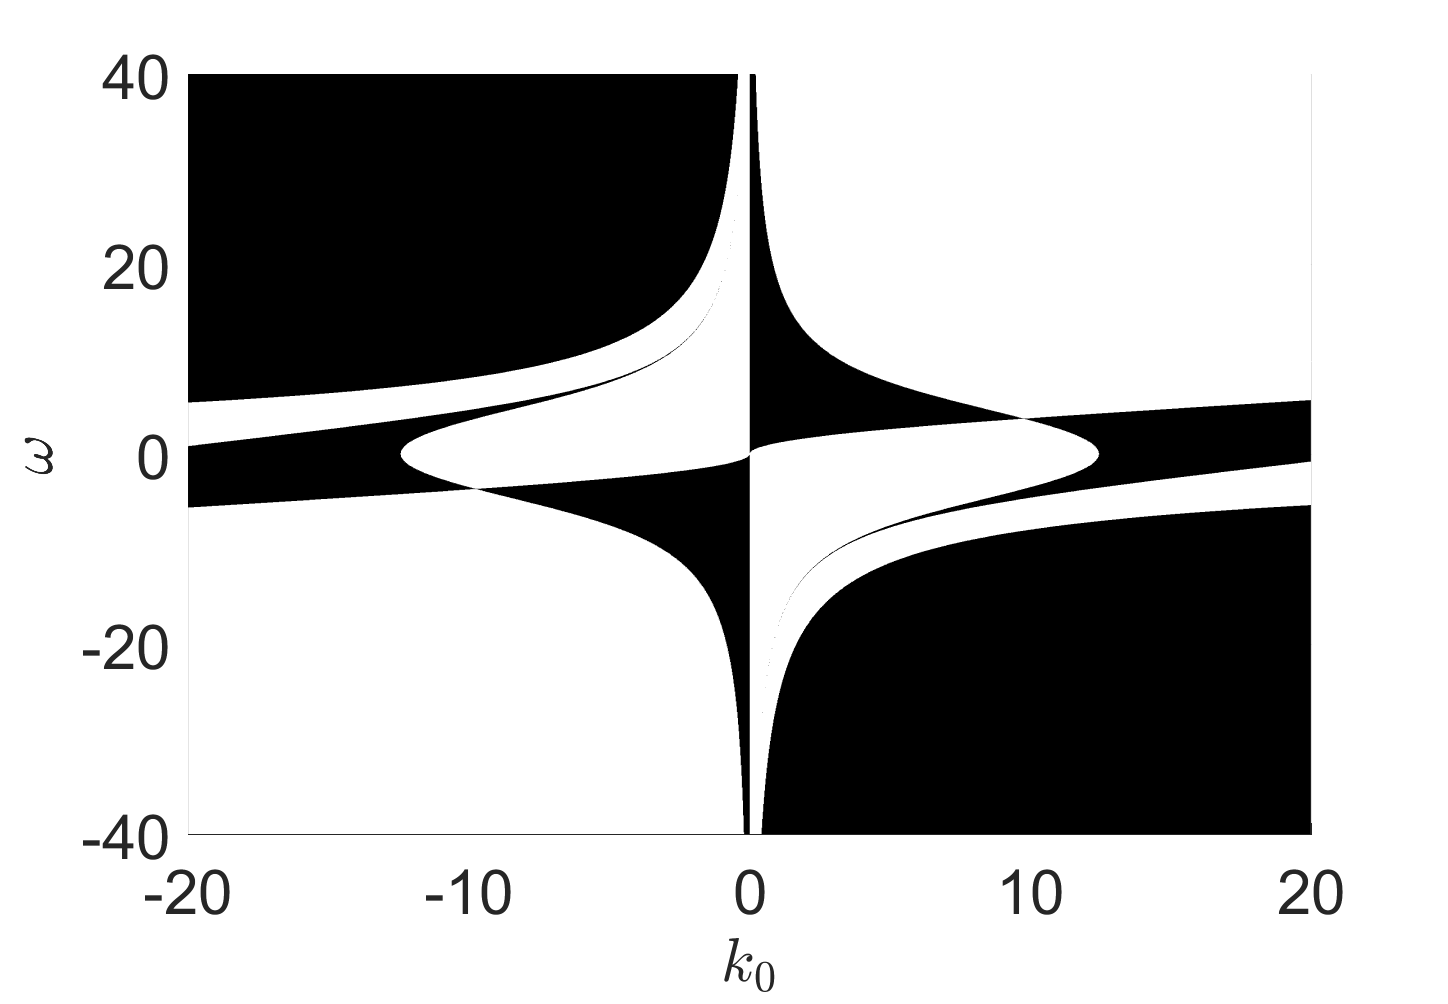
\includegraphics[width=.48\textwidth]{foc_defoc_pos_cut} & 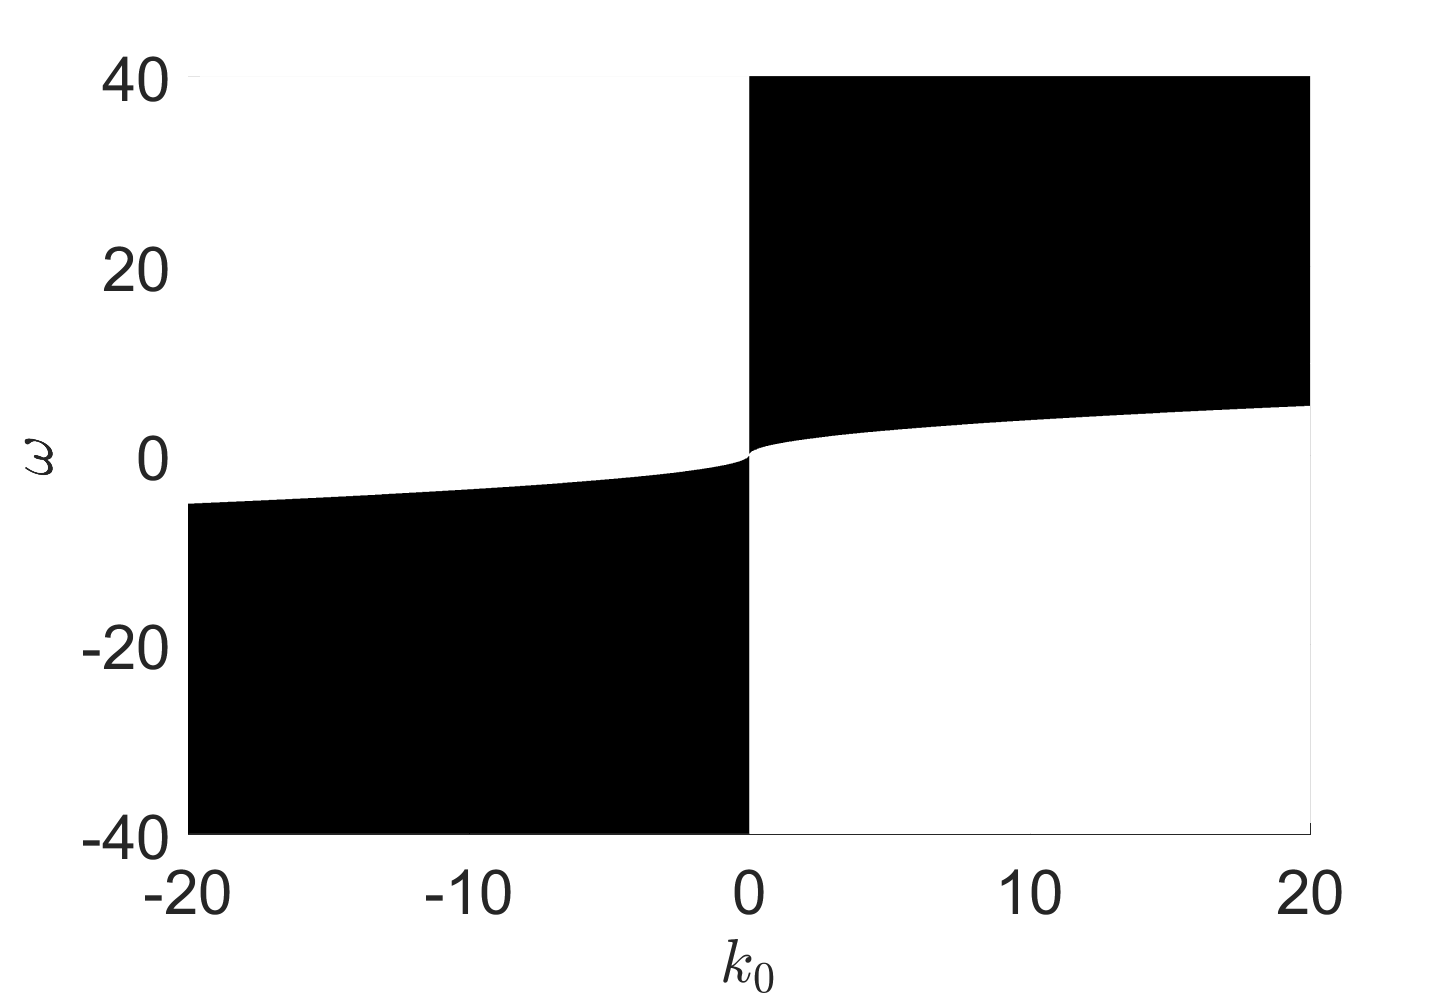
\includegraphics[width=.48\textwidth]{foc_defoc_pos_cut_sig_1en5}\\
(a) & (b)\\
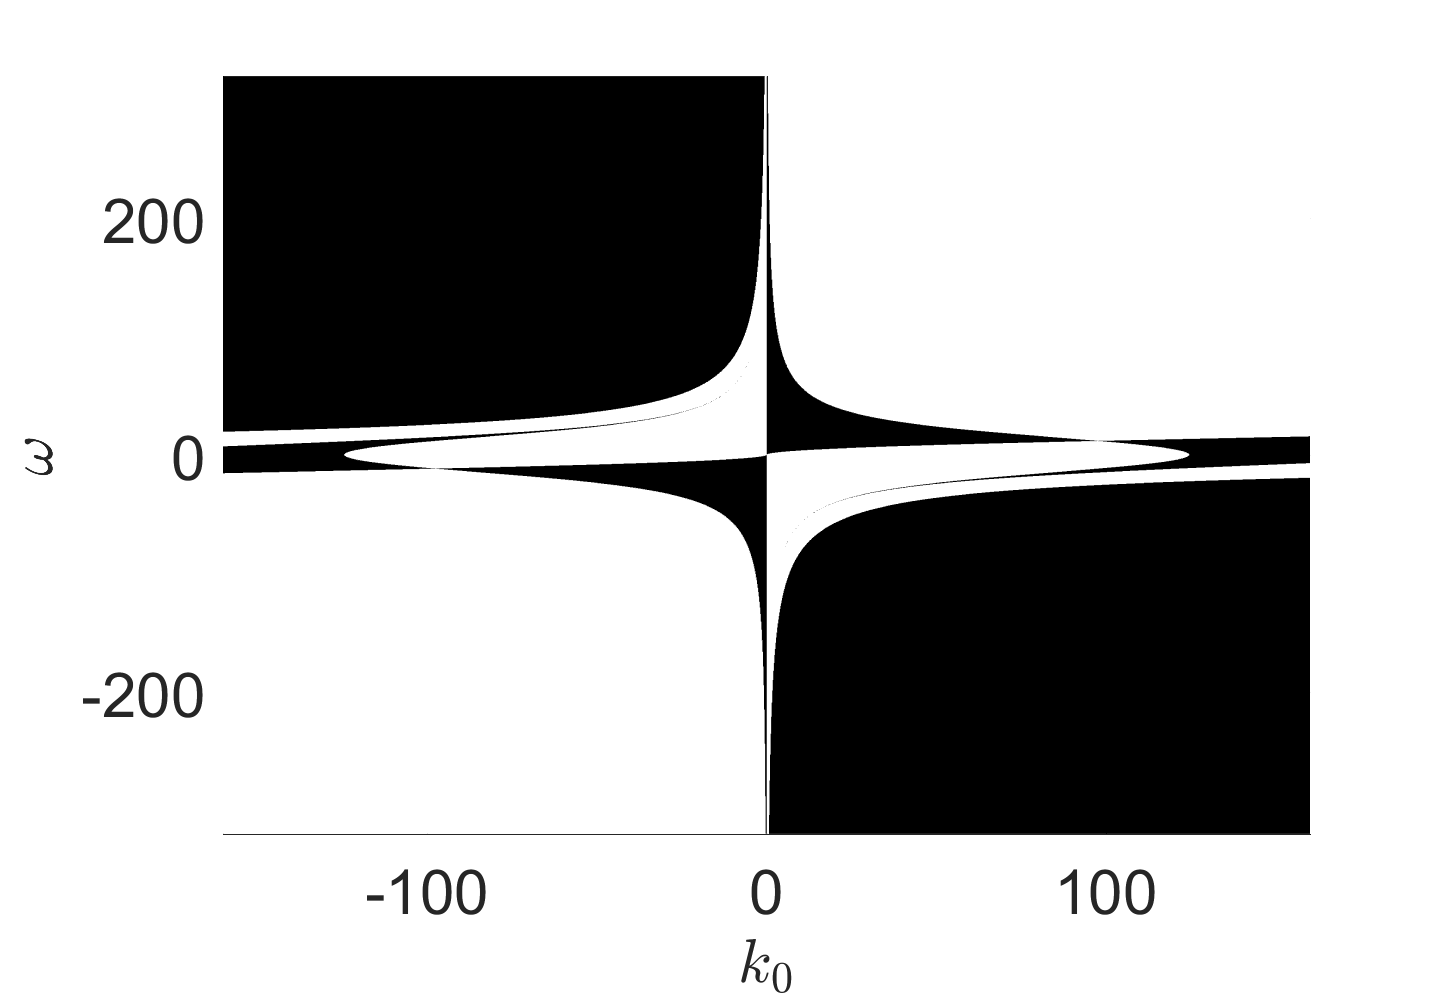
\includegraphics[width=.48\textwidth]{foc_defoc_pos_cut_sig_1en5_wide} & 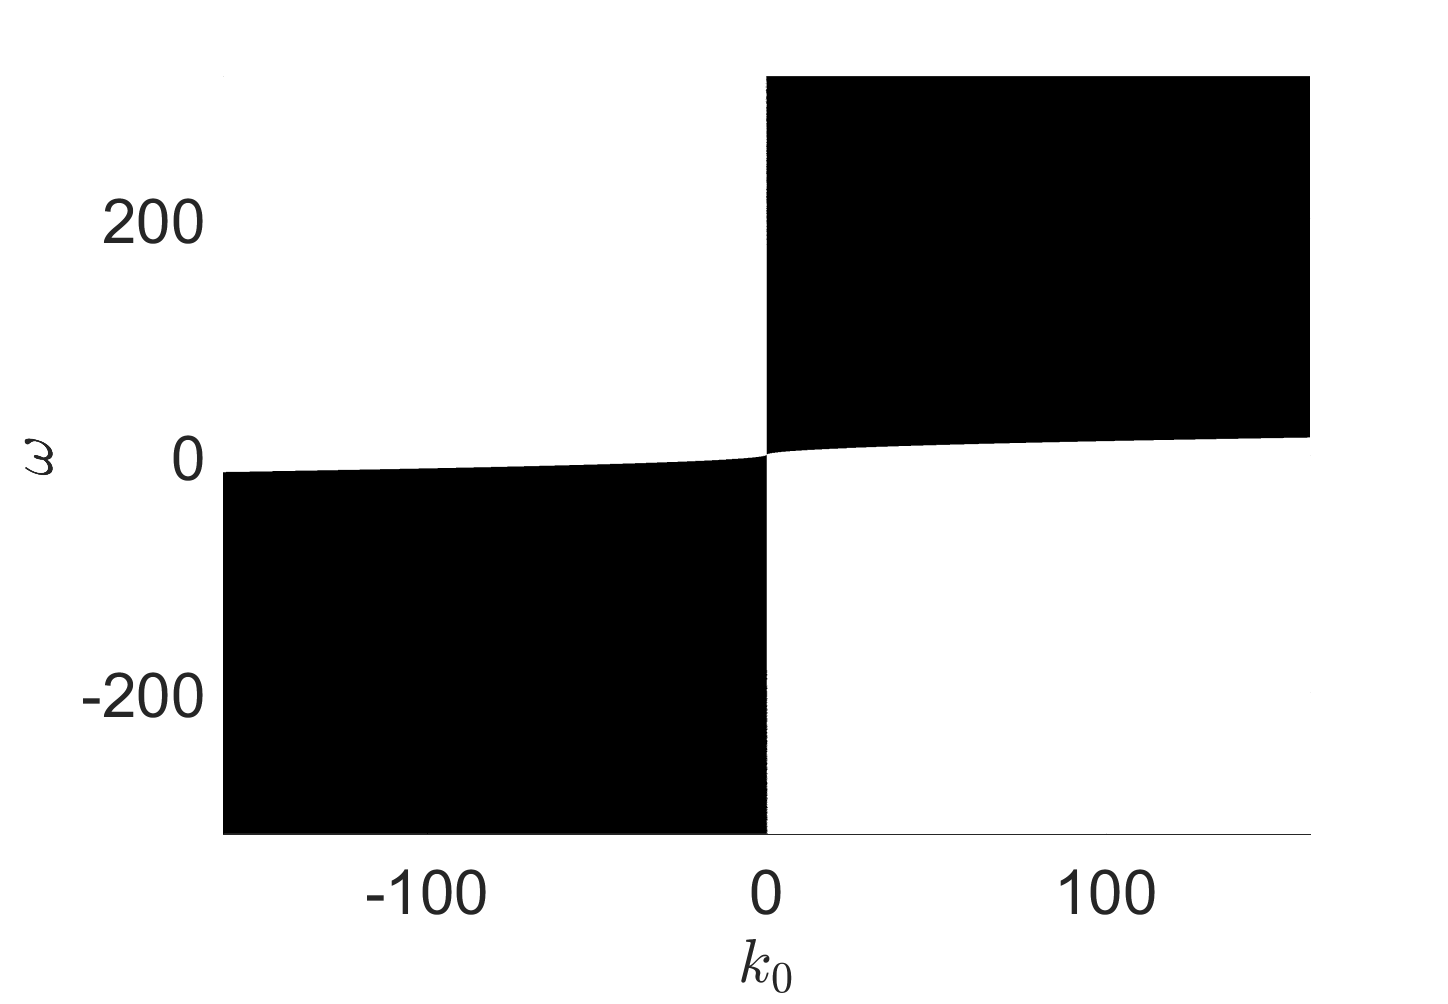
\includegraphics[width=.48\textwidth]{foc_defoc_pos_cut_sig_0_wide}\\
(c) & (d)
\end{tabular}
\caption{\small {\it MIs exist} - white, \small{\it MIs suppressed} - black, for $\tilde{\sigma}=10^{-3}$ (a), $\tilde{\sigma}=10^{-5}$ (b), $\tilde{\sigma}=10^{-5}$ (c), and $\tilde{\sigma}=0$ (d).  Note the change in scale of the axes in (c) and (d) relative to (a) and (b).}
\label{fig:miplot}
\end{figure}

Per our convention of taking the fast phase, $\theta(x,t)$, to be
\[
\theta(x,t) = k_{0}x + \Omega(k_{0},\omega) t,
\]
if $k_{0}\Omega(k_{0},\omega)>0$, then the carrier wave propagates to the left, while if $k_0 \Omega(k_{0},\omega)<0$, it is propagating to the right.  Figures \ref{fig:miplot}(a) and (c) then show that MIs are generally suppressed when the shear current at the surface is co-propagating with respect to the carrier wave with sufficient strength which is inversely related to the carrier wavenumber.  Thus, in order to suppress most MIs, we need either relatively high carrier wave numbers $k_{0}$ for relatively weak shear currents, or relatively strong shear currents for relatively low carrier wave numbers.  The regions in Figures \ref{fig:miplot}(a) and (c) in which counter-propagating sheer currents suppress MIs are more complicated in nature, though one can argue that counter-propagating currents generally exacerbate MIs, especially with increasing shear strength.  
%%%%%%%%%%%%%%%%%%%%%%%%%%%%%%%%%%%%%%%%%%%%%%%%%%%%%%%%%%%%%%%%%%%%%%%%%%%%%%%%%%%
\subsection{Derivation of Velocity Formulas}
In non-dimensional coordinates, the position of a given fluid particle, $(x(t),z(t))$, is defined by the dynamical system 
\begin{align}
\begin{split}
\dot{x} = \omega z + \epsilon \phi_{x}(x,z,t), ~~~~ \dot{z} = \epsilon\phi_{z}(x,z,t),\\
x(0) =x_0,~~~~ z(0)=z_0.
\end{split}
\label{system}
\end{align}
Therefore, in order to track the motion of a fluid particle, both $\phi_x$ and $\phi_z$ must be known throughout the fluid domain.  In order to determine asymptotic formulas for these quantities, let
\begin{equation}
\phi_{x}(x,z,t) = \frac{1}{2\pi}\int_{\mathbb{R}}dk~ e^{ikx} A(k,t)e^{|k|z},
\label{phix}
\end{equation}
\begin{equation}
\phi_{z}(x,z,t) = \frac{1}{2\pi}\int_{\mathbb{R}}dk~ e^{ikx} B(k,t)e^{|k|z}.
\label{phiz}
\end{equation}
Expanding $e^{\epsilon \eta |k|}$ in Equations (\ref{phix}) and (\ref{phiz}) gives
\begin{align}
\left.\phi_{x}\right|_{z=\epsilon\eta} = & \tilde{A}(x,t) - \epsilon\eta\mathcal{H}\pd_{x}\tilde{A} +\mathcal{O}(\epsilon^{2}),\label{phixsurfsol}\\
\left.\phi_{z}\right|_{z=\epsilon\eta} = & \tilde{B}(x,t) - \epsilon\eta\mathcal{H}\pd_{x}\tilde{B} +\mathcal{O}(\epsilon^{2}),\label{phizsurfsol}
\end{align}
where
\[
\tilde{A}(x,t) = \frac{1}{2\pi}\int_{\mathbb{R}}dk~ e^{ikx} A(k,t), ~~~~ \tilde{B}(x,t) = \frac{1}{2\pi}\int_{\mathbb{R}}dk~ e^{ikx} B(k,t).
\]

The surface boundary conditions give
\begin{align*}
\left.\phi_{x}\right|_{z=\epsilon\eta} = & \frac{Q-\epsilon\eta_{x}(\eta_{t}+\epsilon\omega\eta\eta_{x})}{1+\epsilon^{2}\eta_{x}^{2}},\\
\left.\phi_{z}\right|_{z=\epsilon\eta} = & \frac{\eta_{t}+\epsilon \left(Q+\omega\eta\right)\eta_{x}}{1+\epsilon^{2}\eta_{x}^{2}}.
\end{align*}
Substituting the expansions in Equations \eqref{Qexp} and \eqref{nlssurfexp} into these equations and using the results obtained during the derivation of the NLS equation gives 
\begin{align}
\left.\phi_{x}\right|_{z=\epsilon\eta} = & -2\epsilon k_{0}\Omega \left|\eta_{1} \right|^{2} + \left(-s\Omega\eta_{1} + i\epsilon s c_{g}\pd_{\xi}\eta_{1} \right)e^{i\theta} \nonumber \\
& - \epsilon(2s\Omega\eta_{2}+ k_{0}(s\omega-\Omega) \eta_{1}^{2})e^{2i\theta} + \mbox{c.c.} + \mathcal{O}(\epsilon^{2}),\label{phisurfsollhsx}\\
\left.\phi_{z}\right|_{z=\epsilon\eta} = & (i\Omega \eta_{1}+\epsilon c_{g}\pd_{\xi}\eta_{1})e^{i\theta} + i\epsilon(2\Omega\eta_{2} + k_{0}(\omega-s\Omega)\eta_{1}^{2})e^{2i\theta} + \mbox{c.c.} + \mathcal{O}(\epsilon^{2}). \label{phisurfsollhsz}
\end{align}
This motivates the expansions
\begin{align*}
\tilde{A}(x,t) = &  \epsilon \tilde{A}_{01}(\xi,\tau) + \left(\tilde{A}_{10}(\xi,\tau) + \epsilon \tilde{A}_{11}(\xi,\tau)\right)e^{i\theta(x,t)} + \epsilon \tilde{A}_{21}(\xi,\tau)e^{2i\theta(x,t)} + \mbox{c.c.} + \mathcal{O}(\epsilon^{2}),\\
\tilde{B}(x,t) = &  \epsilon \tilde{B}_{01}(\xi,\tau) + \left(\tilde{B}_{10}(\xi,\tau) + \epsilon \tilde{B}_{11}(\xi,\tau)\right)e^{i\theta(x,t)} + \epsilon \tilde{B}_{21}(\xi,\tau)e^{2i\theta(x,t)} + \mbox{c.c.} + \mathcal{O}(\epsilon^{2}).
\end{align*}
Inserting these expansions into Equations \eqref{phixsurfsol} and \eqref{phizsurfsol} and matching powers of $\epsilon$ with the expansions in Equations \eqref{phisurfsollhsx} and \eqref{phisurfsollhsz} gives
\begin{align*}
\tilde{A}_{01} & =  0,\\
\tilde{A}_{10} & =  -s\Omega \eta_{1},\\
\tilde{A}_{11} & =  isc_{g}\pd_{\xi}\eta_{1},\\
\tilde{A}_{21} & =  -(2s\Omega \eta_{2} + k_{0}(s\omega - 2\Omega)\eta_{1}^{2}).
\end{align*}
The expressions for the corresponding terms in $\tilde{B}$ can be found in a similar manner.  

Inverting the Fourier transforms leads to expressions for $A(k,t)$ and $B(k,t)$, which when inserted back into Equations \eqref{phix} and \eqref{phiz} gives 
\[
\phi_{x}(x,z,t) = \tilde{\phi}_{x}(x,z,t) + \mathcal{O}(\epsilon^{2}), ~ \phi_{z}(x,z,t) = \tilde{\phi}_{z}(x,z,t) + \mathcal{O}(\epsilon^{2}),
\]
where 
\begin{equation}
\tilde{\phi}_{x}(x,z,t) = R_{1}(\xi,z,\tau)e^{i\theta} \\+ \epsilon R_{2}(\xi,z,\tau)e^{2i\theta} + \mbox{c.c.},
\label{phixexp}
\end{equation}
\begin{equation}
\tilde{\phi}_{z}(x,z,t) =  \tilde{R}_{1}(\xi,z,\tau)e^{i\theta} \\+ \epsilon \tilde{R}_{2}(\xi,z,\tau)e^{2i\theta} + \mbox{c.c.}.
\label{phizexp}
\end{equation}
Again, while the expansion procedure is straightforward, due to the length of the expressions involved, the details have been omitted.  However, we can still obtain approximations that will be useful later in this paper.  In particular, the leading order behaviors of $R_{1}$ and $\tilde{R}_{1}$, which in turn gives the leading order behaviors of the velocity potentials, are given by 
\begin{align}
R_{1}(\xi,z,\tau) \sim & -\frac{s\Omega}{2\pi}\int_{\mathbb{R}} dk ~ e^{i k \xi} e^{|k_{0}+\epsilon k|z}\hat{\eta}_{1}(k,\tau), \label{roeqx}\\
\tilde{R}_{1}(\xi,z,\tau) \sim & \frac{i\Omega}{2\pi}\int_{\mathbb{R}} dk ~ e^{i k \xi} e^{|k_{0}+\epsilon k|z}\hat{\eta}_{1}(k,\tau). 
\label{roeqz}
\end{align}

%%%%%%%%%%%%%%%%%%%%%%%%%%%%%%%%%%%%%%%%%%%%%%%%%%%%%%%%%%%%%%%%%%%%%%%%%%%%%%%%%%%
\section{The Stokes Drift Velocity}
We now show how our above approximation schemes can be used in to determine how a background shear current modifies the Stokes drift velocity (SDV).  Following the Generalized Lagrangian Mean (GLM) formalism presented in \cite{andrews}, for some quantity $\varphi({\bf x},t)$, given an
Eulerian mean operator $\bar{()}$, we define the Lagrangian mean $\bar{()}^{L}$ at a point ${\bf x}$ relative to the disturbance ${\bf y}({\bf x},t)$ to be  
\[
\bar{\varphi}^{L}({\bf x},t) = \overline{\varphi({\bf x}+{\bf y}({\bf x},t),t)}.
\]
See \cite{kundu} for definitions of Eulerian and Lagrangian coordinates.  Assuming the mapping ${\bf x} + {\bf y}({\bf x},t)$ where
\[
{\bf x} + {\bf y}({\bf x},t) = \left(x+y_{1}(x,z,t),z+y_{2}(x,z,t)\right),
\]
is a diffeomorphism, then a corresponding Lagrangian averaged speed, say $\overline{{\bf u}}^{L}({\bf x},t)$, is defined by the equation
\begin{equation}
\left(\pd_{t} + \overline{{\bf u}}^{L}({\bf x},t)\cdot \nabla_{{\bf x}} \right) \left({\bf x} + {\bf y}({\bf x},t)\right) = {\bf u}\left({\bf x} + {\bf y}({\bf x},t),t\right).
\label{speeddef}
\end{equation}
The other requirements in the GLM formalism are that 
\begin{align*}
\overline{{\bf y}({\bf x},t)} = & \bf{0}, \\
\overline{\overline{{\bf u}}^{L}({\bf x},t)} = & \overline{{\bf u}}^{L}({\bf x},t).
\end{align*}
These assumptions ensure that if we propagate a point ${\bf x}(t)$ with the Lagrangian mean speed $\bar{{\bf u}}^{L}$, thus making ${\bf x}(t)$ a point traveling with the mean flow, then the point ${\bf x}(t) + {\bf y}({\bf x}(t),t)$ is guaranteed to be on a streamline.  Using the above definitions, the Stokes drift, $\varphi^{S}({\bf x},t)$, of a quantity $\varphi$ can be unambiguously defined to be 
\[
\varphi^{S}({\bf x},t) = \overline{\varphi}^{L}({\bf x},t) - \overline{\varphi({\bf x},t)}. 
\]

Throughout the remainder of this paper, the Eulerian average will be given by integration with respect to the fast phase variable $\theta$, i.e.  
\[
\bar{f}(\xi,z,\tau) = \frac{1}{2\pi}\int_{0}^{2\pi} d\theta~ f(\xi,z,\tau,\theta).
\]
Having chosen the averaging operator, one should read the requirement $\overline{{\bf y}}=0$ as in effect a definition of the disturbance.  Equation \eqref{phixexp} and the definition
\[
u({\bf x},t) = \omega z + \epsilon \tilde{\phi}_{x}({\bf x},t) + \mathcal{O}(\epsilon^{3}), 
\]
establish that 
\[
\overline{\phi_{x}}= \mathcal{O}(\epsilon^{2}). 
\]
since there are no mean terms at this order and we average over $\theta$.

Thus, the Eulerian mean of the horizontal velocity, $u({\bf x},t)$, is  
\[
\overline{u}({\bf x},t) = \omega z + \mathcal{O}(\epsilon^{3}).
\]
Correspondingly, we define the Eulerian horizontal fluctuation speed $u'({\bf x},t)$ to be
\[
u'({\bf x},t) = \epsilon\left(e^{i\theta}R_{1} + e^{-i\theta}R_{1}^{\ast} \right)
+  \epsilon^{2}\left( e^{2i\theta}R_{2} + e^{-2i\theta}R_{2}^{\ast}\right)  + \mathcal{O}(\epsilon^{3}),
\]
so that  
\[
u({\bf x},t) = \omega z +  u'({\bf x},t) + \mathcal{O}(\epsilon^{3}).
\]
It is then consistent to suppose that the disturbance ${\bf y}=\mathcal{O}(\epsilon)$, so that, with a slight abuse in notation, we have 
\begin{align}
\overline{u}^{L}({\bf x},t) = & \overline{u({\bf x} + \epsilon {\bf y},t)}, \nonumber \\
= & \overline{\omega (z + \epsilon y_{2}) +  u'({\bf x},t) + \epsilon (y_{1}(\pd_{x}u'+\epsilon\omega\pd_{x}y_{2}) + y_{2} \pd_{z}u') + \mathcal{O}(\epsilon^{3})}, \nonumber \\
= & \omega z + \epsilon \overline{(y_{1}(\pd_{x}u'+\epsilon\omega\pd_{x}y_{2}) + y_{2}\pd_{z}u')} + \mathcal{O}(\epsilon^{3}). \label{lagrandrift}
\end{align}
Note, in order to derive the above formulas, we used a slight modification of the standard GLM transformation in which we used in the shear term $\omega z$ the transformation
\[
\omega(z+\epsilon y_{2}(x+\epsilon y_{1},z,t)) = \omega (z + \epsilon y_{2}) + \epsilon^{2}\omega y_{1}\pd_{x}y_{2} + \mathcal{O}(\epsilon^{3}).
\]
This modification accounts for the dependence of the surface $z=\epsilon \eta$ on the fast phases $\theta$ as seen in Equation \eqref{nlssurfexp}, the impact of which is exacerbated by the $\mathcal{O}(1)$ shear current.    This modification is corroborated by our numerical results presented in the next section.  Using the definition of the SDV then gives the formula 
\[
u^{S} = \bar{u}^{L} - \bar{u} = \epsilon \overline{(y_{1}(\pd_{x}u'+\epsilon\omega\pd_{x}y_{2}) + y_{2}\pd_{z}u' )} + \mathcal{O}(\epsilon^{3}).
\]
Using identical arguments for the vertical velocity $w({\bf x},t)$ gives 
\[
w({\bf x},t) = w'({\bf x},t) + \overline{w}({\bf x},t),
\]
where 
\[
w'({\bf x},t)= \epsilon\left(e^{i\theta}\tilde{R}_{1} + e^{-i\theta}\tilde{R}_{1}^{\ast} \right)
+  \epsilon^{2}\left( e^{2i\theta}\tilde{R}_{2} + e^{-2i\theta}\tilde{R}_{2}^{\ast}\right)  + \mathcal{O}(\epsilon^{3}),
\]
and 
\[
\overline{w}= \mathcal{O}(\epsilon^{3}).  
\]
Therefore, the vertical SDV, $w^{S}$, is given by
\[
w^{S} = \epsilon \overline{(y_{1}\pd_{x}w'+ y_{2}\pd_{z}w')} + \mathcal{O}(\epsilon^{3}).
\]

In order to then determine the disturbance ${\bf y}$, we note that Equation \eqref{speeddef} establishes that
\begin{equation}
\pd_{t}{\bf y} + \omega z \pd_{x}{\bf y} - \omega \bp y_{2}\\ 0 \ep = \bp R_{1}e^{i\theta}+R^{\ast}_{1}e^{-i\theta}\\ \tilde{R}_{1}e^{i\theta}+\tilde{R}^{\ast}_{1}e^{-i\theta} \ep + \mathcal{O}(\epsilon).
\label{vareqn}
\end{equation}
Treating the value $z$ as an Eulerian parameter so that it is independent of time, the method of characteristics gives 
\begin{align*}
y_{1} = & - \frac{i}{k_{0}\omega z + \Omega}\left(R_{1}e^{i\theta} -R^{\ast}_{1}e^{-i\theta} \right) - \frac{\omega}{(k_{0}\omega z + \Omega)^{2}}\left(\tilde{R}_{1}e^{i\theta} + \tilde{R}^{\ast}_{1}e^{-i\theta} \right),\\
y_{2} = & - \frac{i}{k_{0}\omega z + \Omega}\left(\tilde{R}_{1}e^{i\theta} -\tilde{R}^{\ast}_{1}e^{-i\theta} \right).
\end{align*}
Clearly this result is not valid when $z\sim z_{c} \equiv c_{p}(k,\omega)/\omega$, where the phase speed $c_{p}$ is given by 
\[
c_{p}(k_{0},\omega) = -\frac{\Omega(k_{0},\omega)}{k_{0}}.
\]
Again, due to our choice of signs in $\theta(x,t)$, we use the opposite sign on the phase speed so that a positive phase speed $c_{p}$ corresponds to a rightward propagating phase.   We see that $z_{c}$ typefies a kind of stagnation depth in which the carrier wave and the shear profile cancel one another out.  Choosing $k_{0}>0$, we see that as $\omega \gg 1$, $z_{c}\lessapprox -1$, which is, asymptotically speaking, well removed from the surface $z=\epsilon \eta(x,t)$.  However in the case that $\omega \ll -1$, we see that, while $z_{c}$ is always positive, $z_{c}\sim 0$.  Thus, for stronger negative shear values, the expansions above break down around the surface.    Throughout the remainder of the paper, when we look at the case in which $k_{0}\omega <0$, we choose other parameters so as to prevent the surface from overlapping with a critical region in which the GLM expansions above break down. We further explore what happens near $z_{c}$ in the case $k_{0}\omega >0$ at the end of this section.  

Away from the critical depth $z_{c}$, we then use the leading order expansions
\[
R_{1} \sim -s\Omega\eta_{1}e^{|k_{0}|z}, ~ \tilde{R}_{1} \sim i\Omega\eta_{1}e^{|k_{0}|z}, 
\]
so that we get 
\begin{align*}
y_{1} \sim & \frac{-i}{k_{0}\omega z + \Omega}\left(\frac{\omega\Omega}{k_{0}\omega z + \Omega} - s\Omega \right)(\eta_{1}e^{i\theta} - \eta_{1}^{\ast}e^{-i\theta})e^{|k_{0}|z},\\ 
y_{2} \sim & \frac{\Omega}{k_{0}\omega z + \Omega}(\eta_{1}e^{i\theta} + \eta^{\ast}_{1}e^{-i\theta})e^{|k_{0}|z},\\
\p_{x}u' \sim & -i\epsilon|k_{0}|\Omega(\eta_{1}e^{i\theta}-\eta_{1}^{\ast}e^{-i\theta})e^{|k_{0}|z},\\
\pd_{x}w' \sim & - \epsilon k_{0}\Omega(\eta_{1}e^{i\theta}+\eta_{1}^{\ast}e^{-i\theta})e^{|k_{0}|z}.
\end{align*}
Putting these terms together, and using the irrotationality of the Eulerian fluctuation speed, then gives the horizontal component of the SDV to be 
\begin{equation}
u^{S}(x,z,t) = \frac{2\epsilon^{2}\Omega^{2}}{c_{p} - \omega z }\left(1 + \left(\frac{\omega}{|k_{0}|(c_{p} - \omega z )} + 1\right)^{2} \right)|\eta_{1}(\xi,\tau)|^{2}e^{2|k_{0}|z} + \mathcal{O}(\epsilon^{3}), 
\label{sdriftveloc}
\end{equation}
Using similar arguments and expansions, one can show that 
\[
w^{S} = \mathcal{O}(\epsilon^{3}).
\]
Therefore, away from the critical depth $z_{c}$, we can ignore the vertical component of the SDV.  

In the case of a plane-wave solution, the leading-order SDV at the surface can be evaluated in closed form giving  
\begin{equation}
u^{S}(x,z,t) = \frac{2\epsilon^{2}A^{2}\Omega^{2}}{c_{p}-\omega z} \left(1 + \left(\frac{\omega}{|k_{0}|(c_{p} - \omega z )} + 1\right)^{2} \right) e^{2|k_{0}|z} + \mathcal{O}(\epsilon^{3}).
\label{pwavesdrift}
\end{equation}
This expands on the classic result for the SDV over infinitely deep water, and shows how constant shear currents modify the drift velocity.  If the vorticity is assumed to be zero in Equation (\ref{pwavesdrift}) then the classic result
\begin{equation}
u^{S}(x,z,t) \sim a^{2}k_0\sqrt{|k_0|(1+\tilde{\sigma}k_0^2)}~e^{2|k_0|z}, ~ a = 2\epsilon A,
\end{equation}
is obtained for right-moving waves.  Equation (\ref{pwavesdrift}) likewise provides support for the phenomenological choices of how the SDV of a Stokes wave varies in depth made in \cite{breivik}.  There, the classic formula for the SDV was modified by multiplying it by terms like $1/(1+\tilde{c}z)$, where $\tilde{c}$ was then chosen to improve agreements with observed data.  Thus our result provides a physical motivation for the appearance of such terms.  However, while we can put forth a physical mechanism, whether unresolved shear currents near the surface are truly responsible for disagreements between theory and observation is a matter for future work.     

Since we are most interested in surface dynamics, in which $z=\epsilon\eta(x,t)$, we can then use $z\sim 0$, so that the SDV for the Jacobi elliptic function solutions with $\beta=1$ is given by
\[
u^{S}(x,0,t) = -4\epsilon^{2}\kappa^{2}k_{0}\Omega \left|\frac{\alpha_{d}}{\alpha_{nl}}\right| \left(1 + \left(1 - \frac{s\omega}{\Omega} \right)^{2} \right)\phi(\xi;\kappa),
\]
where
\[
\phi(\xi;\kappa) = \left\{\ba{rl} \mbox{cn}^2(\xi;\kappa), & \alpha_{d}/\alpha_{nl}>0, \\  \mbox{sn}^2(\xi;\kappa), & \alpha_{d}/\alpha_{nl}<0.\ea \right.
\]
Defining the parameter
\[
\tilde{u}^{S}(k_{0},\omega) = -4 k_{0}\Omega(k_{0},\omega) \left|\frac{\alpha_{d}(k_{0},\omega)}{\alpha_{nl}(k_{0},\omega)}\right|\left(1 + \left(1 - \frac{s\omega}{\Omega(k_{0},\omega)} \right)^{2} \right),
\]
and choosing the positive branch of the dispersion relationship, Figure \ref{fig:sdriftmag_sign} shows that this term exhibits a wide variation in magnitude.  The curves along which the largest magnitudes are seen correspond to the level set $\alpha_{nl}(k_{0},\omega)=0$.  Thus, for the class of Jacobi elliptic solutions, there appears to be a kind of nonlinear resonance between the shear current and the carrier wave.  We point out that along this curve though, the assumptions we used to derive the NLS equation are no longer valid.  Therefore, more work should be done to better elucidate the affiliated dynamics associated with parameter choices defining said curve.  Throughout the remainder of this paper, we choose parameter values that do not place us too near the zero set of $\alpha_{nl}(k_{0},\omega)=0$.
\begin{figure}
\centering
\begin{tabular}{c}
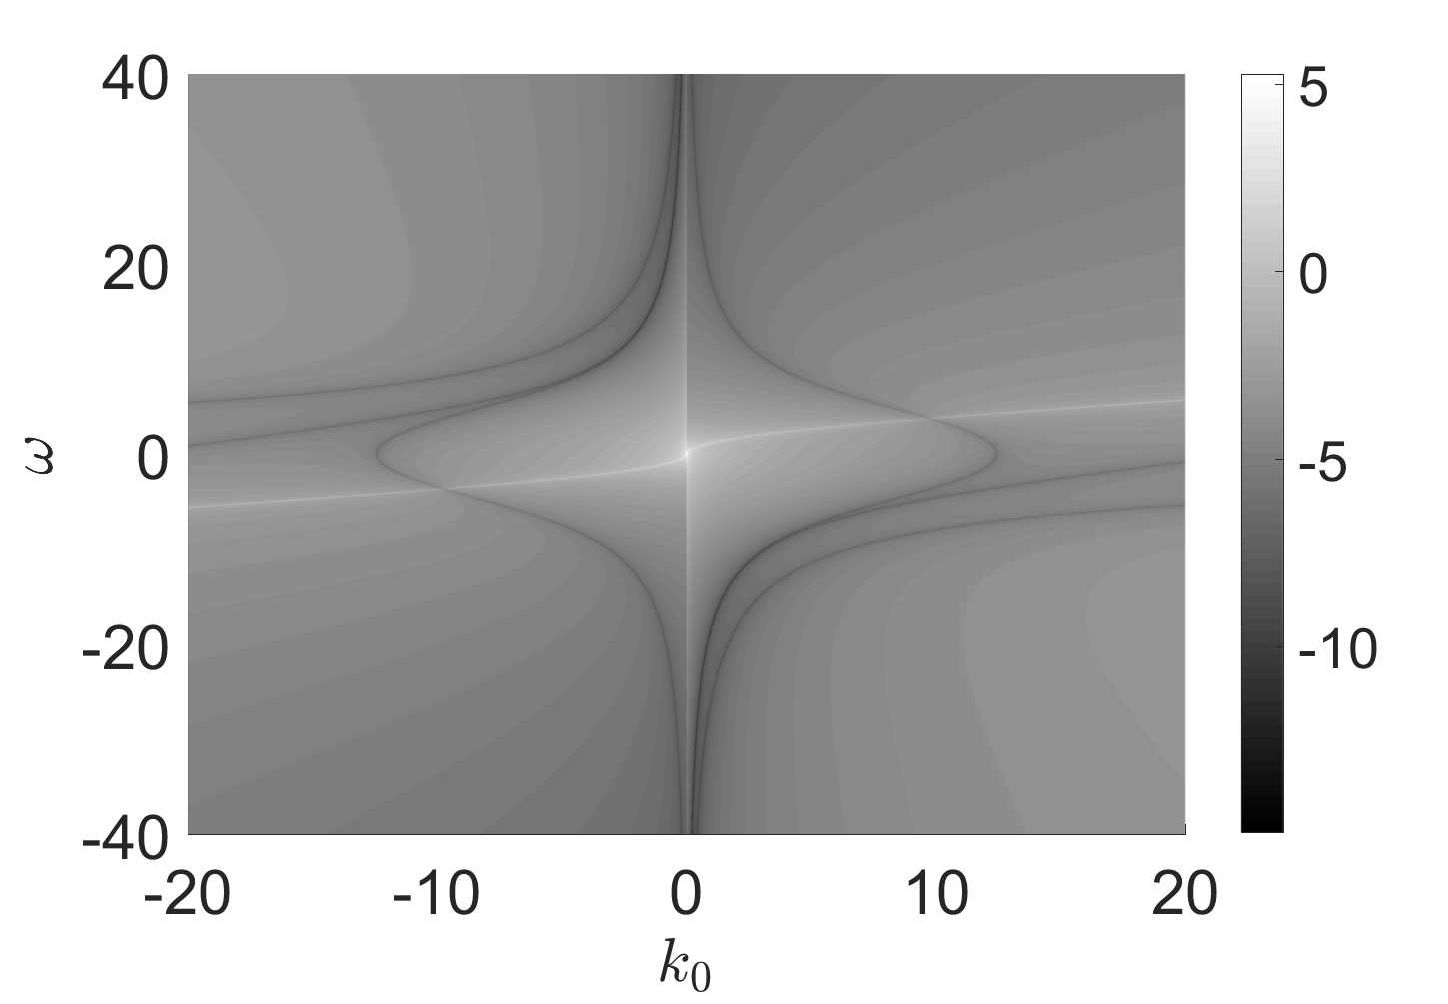
\includegraphics[width=.48\textwidth]{us_magnitude} 
\end{tabular}
\caption{\small Log plot of the SVD $\tilde{u}^{S}(k_{0},\omega)$.  The curves along which $\tilde{u}^{S}(k_{0},\omega)=0$ mirror the transistions between MI stable and unstable regions seen in Figure \ref{fig:miplot}.  The Stokes drift is most augmented along the curves correpsonding to $\alpha_{nl}(k_{0},\omega)=0$.  }
\label{fig:sdriftmag_sign}
\end{figure} 

To get a more detailed understanding of how the SDV depends on the shear current strength, we choose $k_{0}=1$ and use the positive branch of the dispersion relationship.  Figure \ref{fig:stksdrfcomp} contains plots of $\tilde{u}^{S}(1,\omega)$ for $-1\leq \omega\leq 4$, $-1\leq \omega \leq 1.1$, and $1.2\le\omega\le4$.  We choose these particular ranges of shear values to in particular examine the behavior of $\tilde{u}^{S}$ around the resonance curve seen in Figure \ref{fig:sdriftmag_sign}.  The singularity seen in Figure \ref{fig:stksdrfcomp} (a) corresponds to the value $\omega$ such that $\alpha_{nl}(1;\omega)=0$, namely $\omega\approx1.1550$.  Figure \ref{fig:stksdrfcomp} (b) shows the focusing side and that increasing the shear strength increases the Stokes drift velocity.  Figure \ref{fig:stksdrfcomp} (c) shows that this relationship is reversed on the defocusing side.  
\begin{figure}
\centering
\begin{tabular}{ccc}
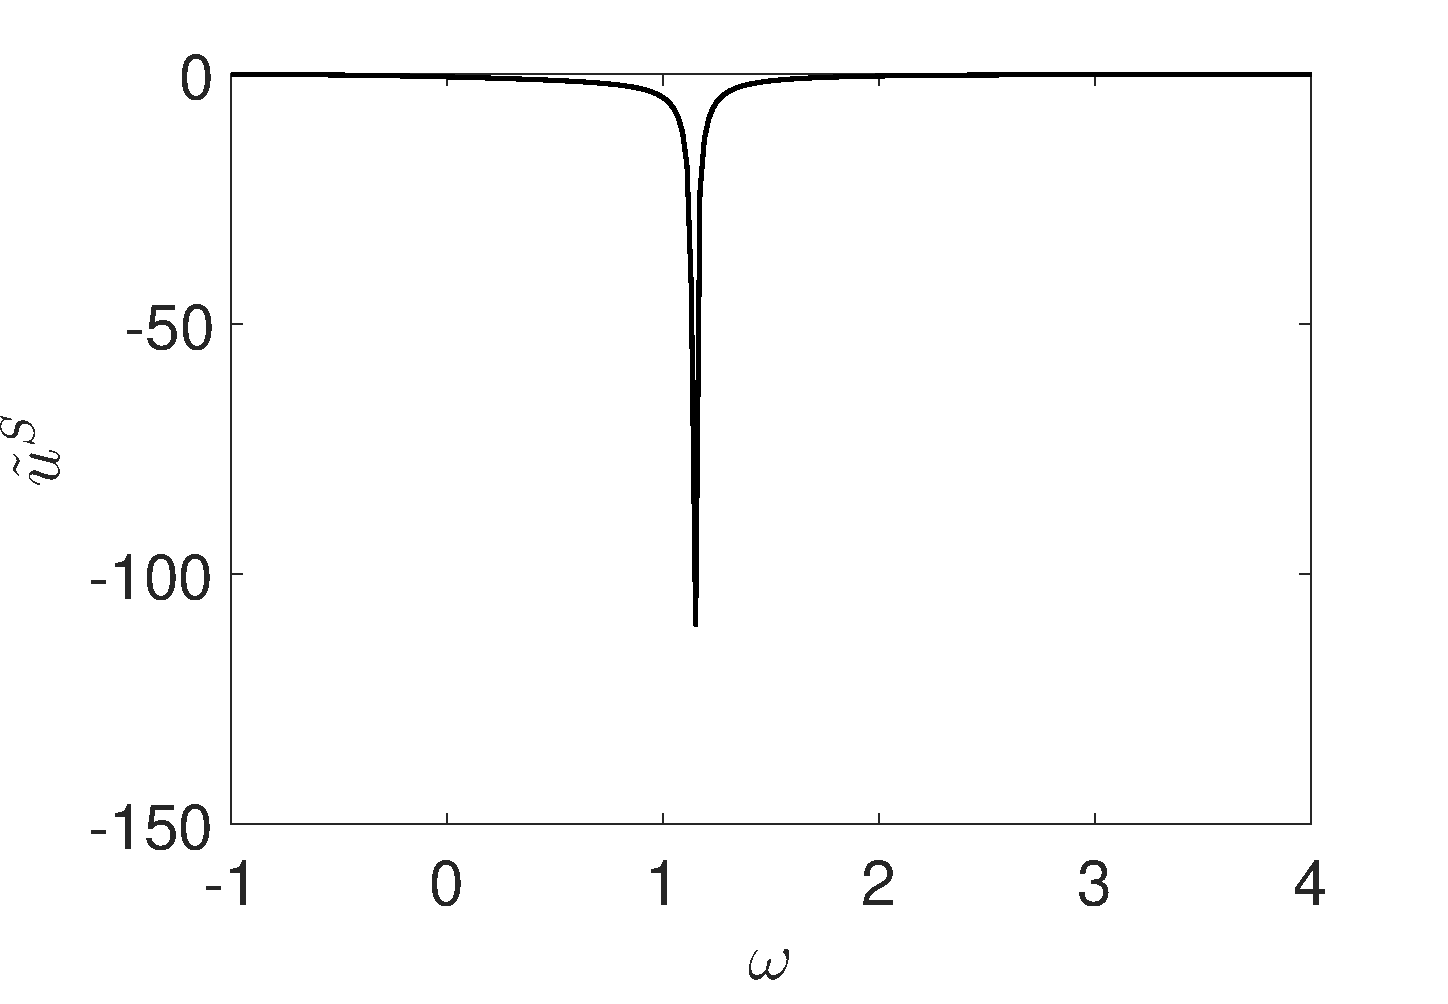
\includegraphics[width=.32\textwidth]{us_wide_range} & 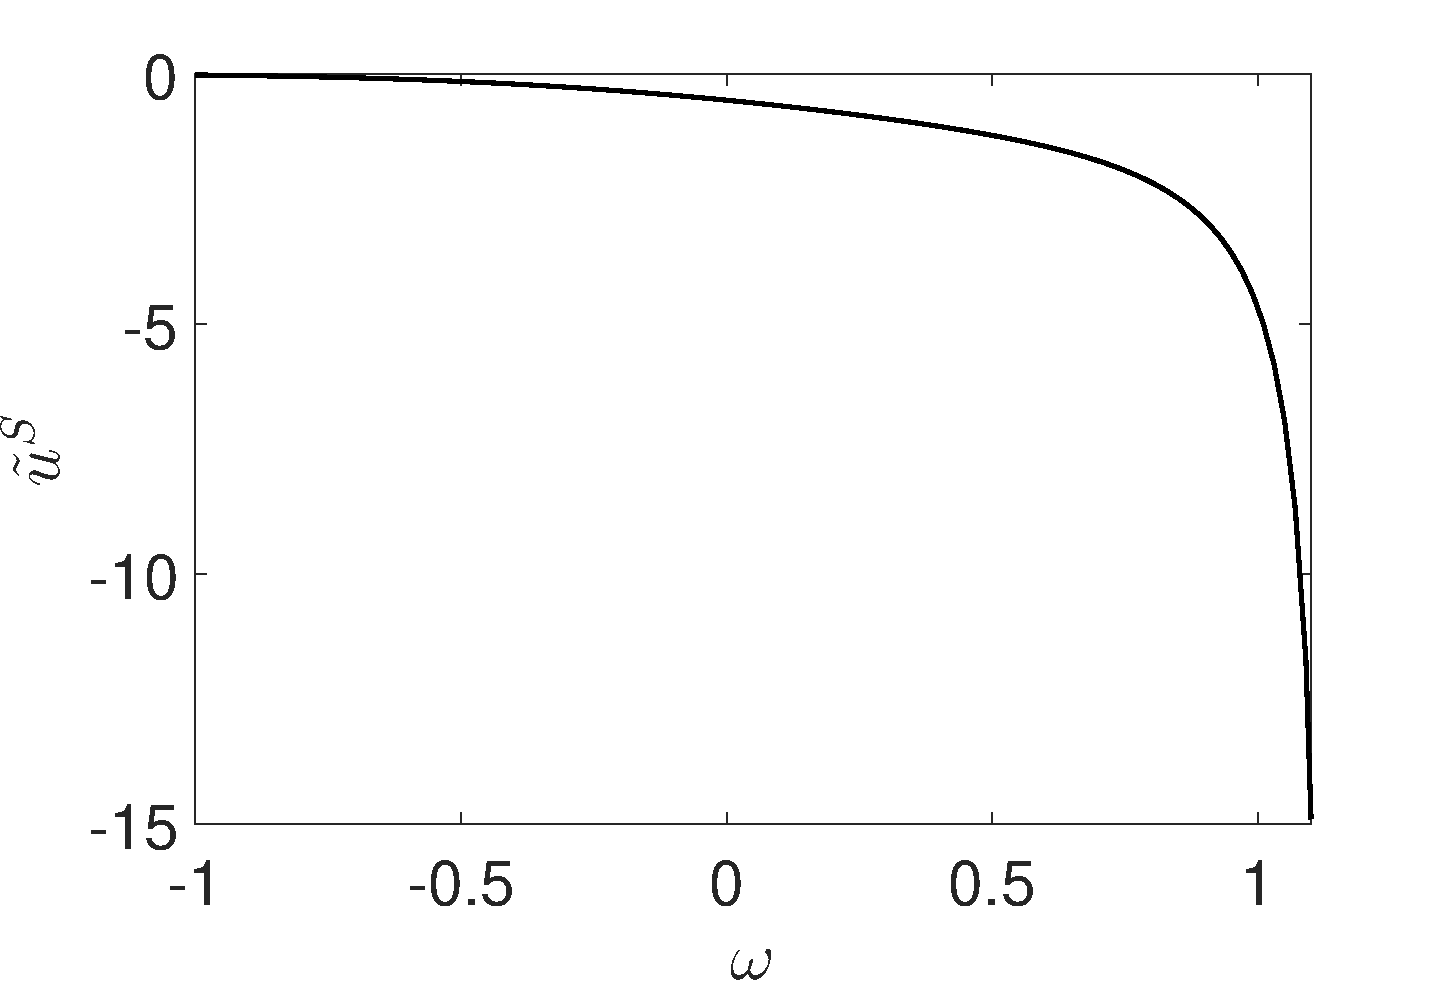
\includegraphics[width=.32\textwidth]{us_n1_to_1pt1} & 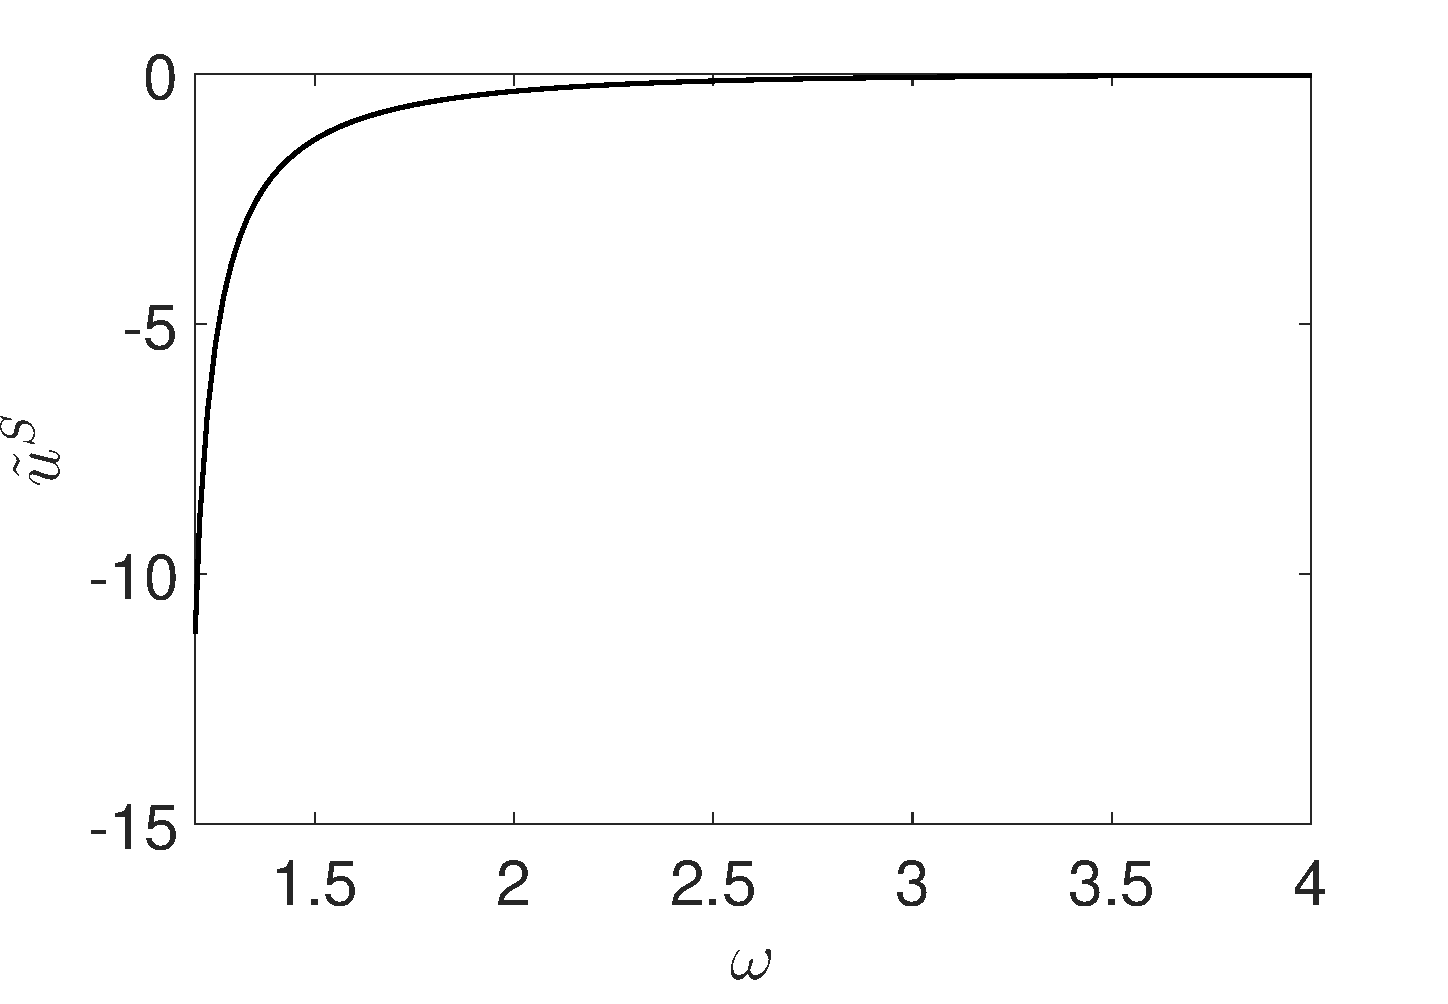
\includegraphics[width=.32\textwidth]{us_1pt2_to_4}\\
(a) & (b) & (c)
\end{tabular}
\caption{\small Plots of $\tilde{u}^{S}(1,\omega)$ for $-1\leq \omega \leq 4$ (a), $-1\leq \omega \leq 1.12$ (b), and $1.17\leq \omega \leq 4$ (c).  Note, $\alpha_{nl}(1;1.1550)=0$.  The figure shows that the magnitude of the SDV increases with increasing shear on the focusing side of the singularity (b), and decreases with increasing shear on the defocusing side (c).}
\label{fig:stksdrfcomp}
\end{figure}

Next, we address the question of the Lagrangian drift velocity (LDV) $\bar{u}^{L}(x,z,t)$ at or near the surface $z=\epsilon \eta$.  Using Equation \eqref{meansurf} for the mean surface displacement term $\eta_{0}$, Equation \eqref{sdriftveloc} for the SDV, and Equation \eqref{lagrandrift} for $\bar{u}^{L}$, the leading-order LDV at the surface $z=\epsilon \eta$, say $\bar{u}^{L,s}(x,t)$, is given by
\[
\bar{u}^{L,s}(x,t) = \epsilon^{2} u^{L}_{p}(k_{0},\omega)|\eta_{1}(\xi,\tau)|^{2} + \mathcal{O}(\epsilon^{3}),
\]
where the scaling factor $u^{L}_{p}$ is given by 
\[
u^{L}_{p}(k_{0},\omega) =  \frac{ \omega^{2}(2s\Omega(k_{0},\omega) - \omega)}{1+\omega c_{g}(k_{0},\omega)} - 2k_{0}\Omega(k_{0},\omega)\left(1 + \left(1 - \frac{s\omega}{\Omega(k_{0},\omega)} \right)^{2}\right). 
\]
The LDV determines the mean horizontal velocity of a particle at or near the surface, and this is then controlled by the magnitude of the solution to the NLS equation we study and the magnitude of $u^{L}_{p}$.  Of particular interest given the puzzling results on the existence of drift quenching Eulerian counterflows \cite{monismith,smith}, we can also then determine vorticity values $\omega$ for a given wavenumber $k_{0}$ such that $u^{L}_{p}(k_{0},\omega) =0$, which corresponds to the presence of an Eulerian counterflow which counters the effect of the SDV.  We plot this zero level set for $0\leq k_{0}\leq 20$ in Figure \ref{fig:zerodriftk0}.  As can be seen, shear strengths which contribute to the suppression of particle drift are always counter-propagating relative to a positively elevated surface.  
\begin{figure}
\centering
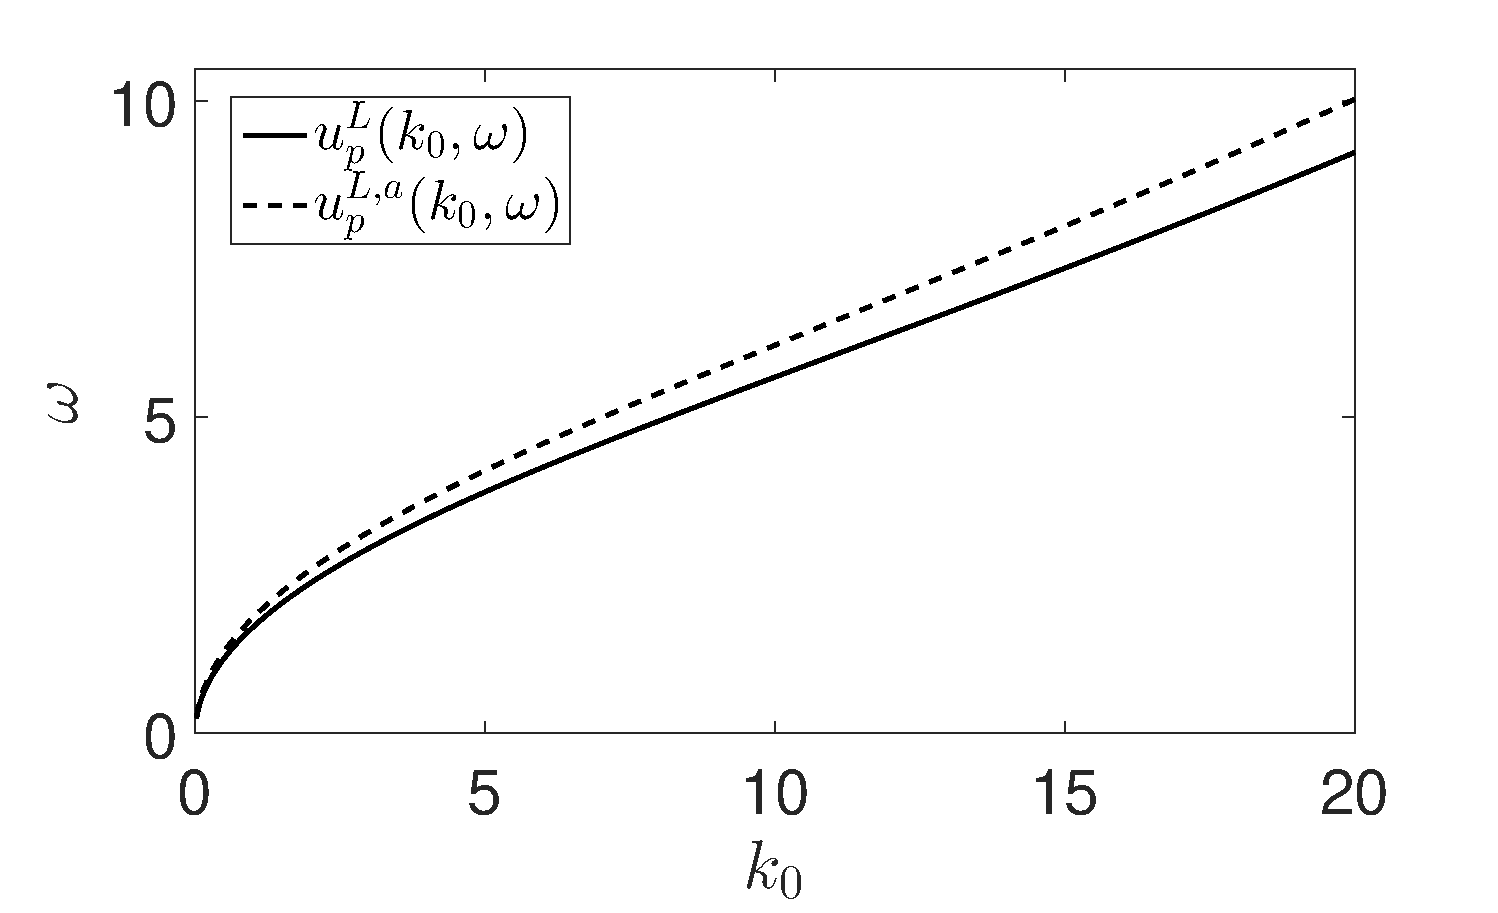
\includegraphics[width=.55\textwidth]{zero_return_shear}
\caption{\small Plot of the zero set $u^{L}_{p}(k_{0},\omega)=0$.}
\label{fig:zerodriftk0}
\end{figure}

At this point, we note that the modification to GLM used above is only relevant near the oscillating surface $z=\epsilon \eta$.  Away from the surface we use the unmodified GLM method, so that the formula we get for the SDV, say $u^{S,a}$, is 
\[
u^{S,a}(k_{0},\omega) =  \frac{2\epsilon^{2} \Omega^{2}}{c_{p}-\omega z} \left( 2 +  \frac{\omega}{|k_{0}|(c_{p} - \omega z )} \right)\left|\eta_{1}\right|^{2} e^{2|k_{0}|z} + \mathcal{O}(\epsilon^{3}). 
\]
Comparing to the formula derived above, we see the difference between the two formulas is 
\[
u^{S} - u^{S,a} =  \frac{2\epsilon^{2} \Omega^{2}\omega}{|k_{0}|\left(c_{p}-\omega z\right)^{2}}\left(1 + \frac{\omega}{|k_{0}|\left(c_{p}-\omega z\right)}\right) \left|\eta_{1}\right|^{2} e^{2|k_{0}|z} + \mathcal{O}(\epsilon^{3}),
\]
which essentially vanishes if $\omega=0$ and decays like $e^{2|k_{0}|z}/z^{2}$ as $z\rightarrow -\infty$.  Thus, we see that we should use different estimates for the SVD depending on whether one looks close to the surface $z=\epsilon \eta$ or if one looks at a relatively deep point $|z|\gg |z_{c}|$. 

%As one would expect, our modification of the GLM approach alters the computation of the SDV, which in turn then would markedly shift where the zero set of $u^{L,a}_{p}(k_{0},\omega)$ appears relative to the zero set of $u^{L}_{p}(k_{0},\omega)$.  This is illustrated by comparing the two curves plotted in Figure \ref{fig:zerodriftk0}.  As shown in subsequent sections, the numerical simulations we have developed confirm the prediction of quenched surface drift velocity given by finding $u^{L}_{p}(k_{0},\omega)=0$, thereby validating our generalization of the GLM methodology.  

\subsection{Flow Near the Critical Depth $z_{c}$}
Taking $k_{0}\omega >0$ so that $-\infty<z_{c}<-1$, it is illuminating to begin to examine what the mean and fluctuation components of the flow are near the critical depth $z_{c}$.  Introducing the interior variable $\tilde{z}$ where
$$
\tilde{z} = \frac{1}{\epsilon^{2}}\left(z - z_{c} \right), 
$$
if we repeat the steps used to derive Equation \eqref{vareqn}, then we get that
\begin{equation}
\pd_{t}{\bf y} + \omega z_{c} \pd_{x}{\bf y}  + w^{S}\pd_{\tilde{z}}{\bf y} - \omega \bp y_{2}\\ 0 \ep = \bp R_{1}e^{i\theta}+R^{\ast}_{1}e^{-i\theta}\\ \tilde{R}_{1}e^{i\theta}+\tilde{R}^{\ast}_{1}e^{-i\theta} \ep + \mathcal{O}(\epsilon).
\label{modvareqn}
\end{equation}
 Note, while we showed above that $w^{S}=\mathcal{O}(\epsilon^{3})$, this was a direct consequence of the form of the solutions of the variations $y_{j}$.  For $z\sim z_{c}$ this need no longer be the case, and we revert back to the more general statement that  $w^{S}=\mathcal{O}(\epsilon^{2})$, which is why we set the width of the layer around $z_{c}$ to be $\mathcal{O}(\epsilon^{2})$.  We therefore see that a relatively thin boundary layer should emerge in which the vertical SVD becomes more significant.  
 
 We further see that by including the term $w^{S}$ in Equation \eqref{modvareqn}, we have made the problem nonlinear, thus allowing for more complicated dynamics within the critical region around $z_{c}$.  To wit, by using the ansatze 
 \[
 y_{1} = y_{11}(\xi,\tau,\tilde{z})e^{i\theta} + y_{11}^{\ast}(\xi,\tau,\tilde{z})e^{-i\theta} + \cdots, ~  y_{2} = y_{21}(\xi,\tau,\tilde{z})e^{i\theta} + y_{21}^{\ast}(\xi,\tau,\tilde{z})e^{-i\theta} + \cdots,
 \]
 we can show that Equation \eqref{modvareqn} becomes 
 \begin{align*}
 -\omega y_{21} + 2k_{0}\left(-\mbox{Im}\left\{y_{11}^{\ast}\tilde{R}_{1}\right\}+s\mbox{Re}\left\{y_{21}^{\ast}\tilde{R}_{1}\right\}\right)\pd_{\tilde{z}}y_{11} = & R_{1}\\
2k_{0}\left(-\mbox{Im}\left\{y_{11}^{\ast}\tilde{R}_{1}\right\}+s\mbox{Re}\left\{y_{21}^{\ast}\tilde{R}_{1}\right\}\right)\pd_{\tilde{z}}y_{21} = & \tilde{R}_{1}.
 \end{align*}
 Separating into real and imaginary parts makes this a four-dimensional nonlinear system to solve.  However, a bit of manipulation, and noting that $R_{1}$ and $\tilde{R}_{1}$ are to leading order independent of $\tilde{z}$, leads to the constraint
 \[
 R_{1}y_{21} + \frac{\omega}{2}y_{21}^{2} = \tilde{R}_{1}y_{11} + \tilde{C}, ~ \tilde{C} = \tilde{C}(\xi,\tau),
 \]
 thus allowing for a reduction of the system by two dimensions.  Letting 
 \[
 y_{21} = y_{21}^{(r)} + i y_{21}^{(i)},
 \]
 we can then readily show that 
 \[
 y^{(i)}_{21} = \frac{\bar{C} + \tilde{R}_{1}^{(i)}y_{21}^{(r)}}{\tilde{R}_{1}^{(r)}}, ~ \bar{C} = \bar{C}(\xi,\tau),
 \]
 and then 
 \[
 \tilde{\tilde{C}} y_{21}^{(r)} + \frac{\alpha_{0}}{2}\left(y_{21}^{(r)}\right)^{2} + \frac{\alpha_{1}}{3}\left(y_{21}^{(r)}\right)^{3} = \frac{\tilde{R}_{1}^{(r)}}{2k_{0}}\tilde{z} + \tilde{D},
 \]
where $\tilde{\tilde{C}}$ and $\tilde{D}$ are real value constants depending only on the slow variables $\xi$ and $\tau$, while $\alpha_{0}$ and $\alpha_{1}$ are real valued constants which depend on the physical parameters of the problem.  Note, details are ommitted for brevity.  

As we see then, since this is a cubic equation, we are always guaranteed at least one real root for all values of $\tilde{z}$, thus permitting for $y_{21}$ to in principal be computed, which in turn gives us $y_{11}$ and thus the fluctuation about the mean in the critical layer around $z_{c}$.  While addressing further details, such as asymptotically matching across the layer, will be left for future work, our preliminary analysis shows that a background shear approprialately aligned to the carrier wave, i.e. when $k_{0}\omega >0$, creates a relatively sharp boundary layer in which the mean transport properties and fluctuation dynamics are markedly altered in comparison to the rest of the fluid.  The impact of this on flow properties throughout the bulk of the fluid is also a question of future research. 
%%%%%%%%%%%%%%%%%%%%%%%%%%%%%%%%%%%%%%%%%%%%%%%%%%%%%%%%%%%%%%%%%%%%%%%%%%%%%%%%%%%
%%%%%%%%%%%%%%%%%%%%%%%%%%%%%%%%%%%%%%%%%%%%%%%%%%%%%%%%%%%%%%%%%%%%%%%%%%%%%%%%%%%
\section{Numerical Results}
In order to determine the particle paths, the system in Equation (\ref{system}) must be solved.  However, since the NLS solutions are in terms of the coordinates $\xi$ and $\tau$, the dynamical system
\[
\frac{d \xi_{s}}{d\tau} =  \frac{c_{g}}{\epsilon} + \frac{\omega}{\epsilon}z_{s} + \tilde{\phi}_{x}(\xi_{s},z_{s}), ~~~~ \frac{dz_{s}}{d\tau} = \frac{1}{\epsilon} \tilde{\phi}_{z}(\xi_{s},z_{s}),
\]
\[
\xi_s(0)=\xi_0, ~~~~ z_s(0)=z_0,
\]
where the potentials $\tilde{\phi}_{x}$ and $\tilde{\phi}_{z}$ are found in Equations \eqref{phixexp} and \eqref{phizexp} respectively must be solved.  Given our focus on determining particle paths at the surface, we approximate the surface profile by
\[
z_{s}(t) = \epsilon \tilde{\eta}(\xi_{s}(t),t). 
\]
Thus, the coupled system of ODEs is reduced to a single, nonlinear, scalar equation
\[
\frac{d \xi_{s}}{d\tau} =  \frac{c_{g}}{\epsilon} + \omega\tilde{\eta}(\xi_{s},t) + \tilde{\phi}_{x}(\xi_{s},\epsilon\tilde{\eta}),
\]
\[
\xi_s(0)=\xi_0.
\]
We use a fourth-order Runge-Kutta scheme with a time step of $\delta \tau = 5\times10^{-4}$ to solve this initial-value problem.  

For the Jacobi elliptic function solutions, we choose the initial tracer position to be 
\[
\xi_{s}(0) = \frac{K(\kappa)}{128}, ~ z_{s}(0) = \epsilon \tilde{\eta}(\xi_{s}(0),0),
\]
where $K(\kappa)$ is the complete elliptic integral of the first kind and $\tilde{\eta}$ is defined by Equation \eqref{nlssurfexp}.  For the plane wave solutions, we chose $\xi_s(0)=10/128$ so the initial positions are comparable across the different classes of solutions.  We take the positive branch of the dispersion relationship, which implies that $k_{0}>0$ corresponds to a left-moving-carrier wave.  We choose $k_{0}=1$ for the plane-wave solutions.  In the case of the Jacobi elliptic solutions to the NLS equation, we choose the integer $m$ to be 
\[
m = \left\lfloor \frac{2K(\kappa)}{\pi \epsilon}\right\rfloor,
\]
so that, using Equation \eqref{jacwavnum}, $k_{0}\approx 1$.  In practice, $k_{0}\approx0.98$ or $0.99$.  The results for the tracer position in physical coordinates, $(x_{s}(t),z_{s}(t))$, are found using the transformations 
\[
x_{s}(t) = \frac{\xi_{s}(\tau)}{\epsilon}-\frac{c_{g}\tau}{\epsilon^{2}}, ~~~~ t = \frac{\tau}{\epsilon^{2}}.
\]
Fourier transforms and their inverses are computed numerically using the fast Fourier transform. 

Finally, note that the expansions in \eqref{phixexp} and \eqref{phizexp}, and the associated approximations in \eqref{roeqx} and \eqref{roeqz}, show that the strength of the velocity field is largely determined by the magnitude of the solution to the NLS equation given by $\eta_{1}$.  In the case of the Jacobi elliptic function solutions, controlling for the elliptic modulus $\kappa$, the term $\sqrt{2|\alpha_{d}/\alpha_{nl}|}$ is the most significant contribution to the magnitude of $\eta_{1}$ since we have fixed $\beta=1$; see Equations \eqref{cnsolns} and \eqref{snsolns}.  Figure \ref{fig:ampcomps} contains plots of $\sqrt{2|\alpha_{d}/\alpha_{nl}|}$ versus $\omega$ for $k_0=1$.
\begin{figure}
\centering
\begin{tabular}{ccc}
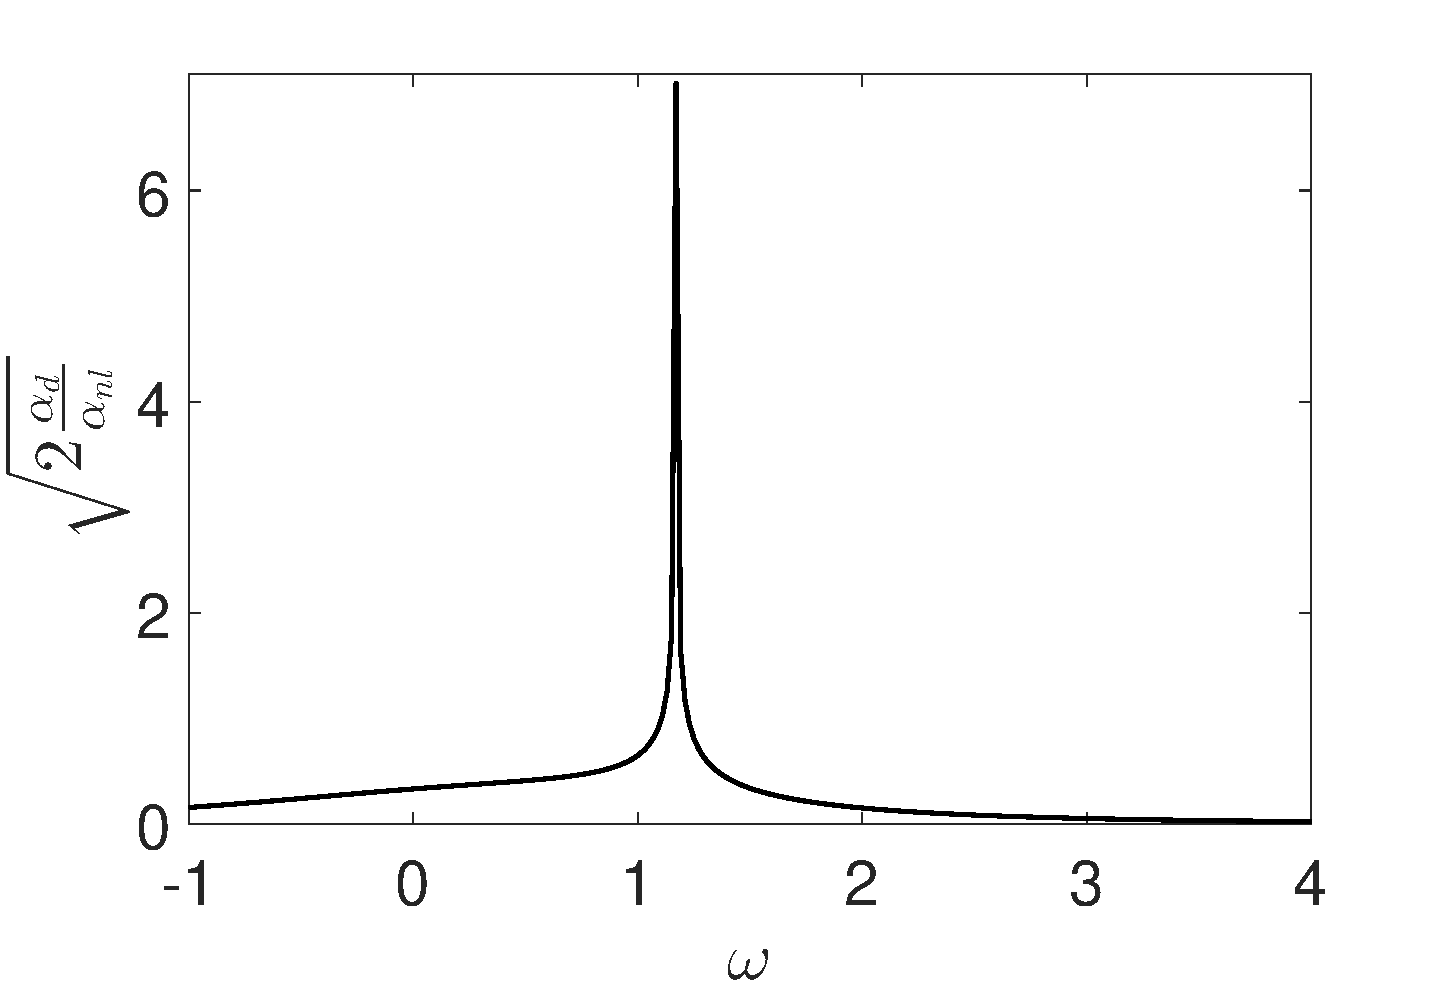
\includegraphics[width=.32\textwidth]{amp_factor_k0_1_wide_range} & 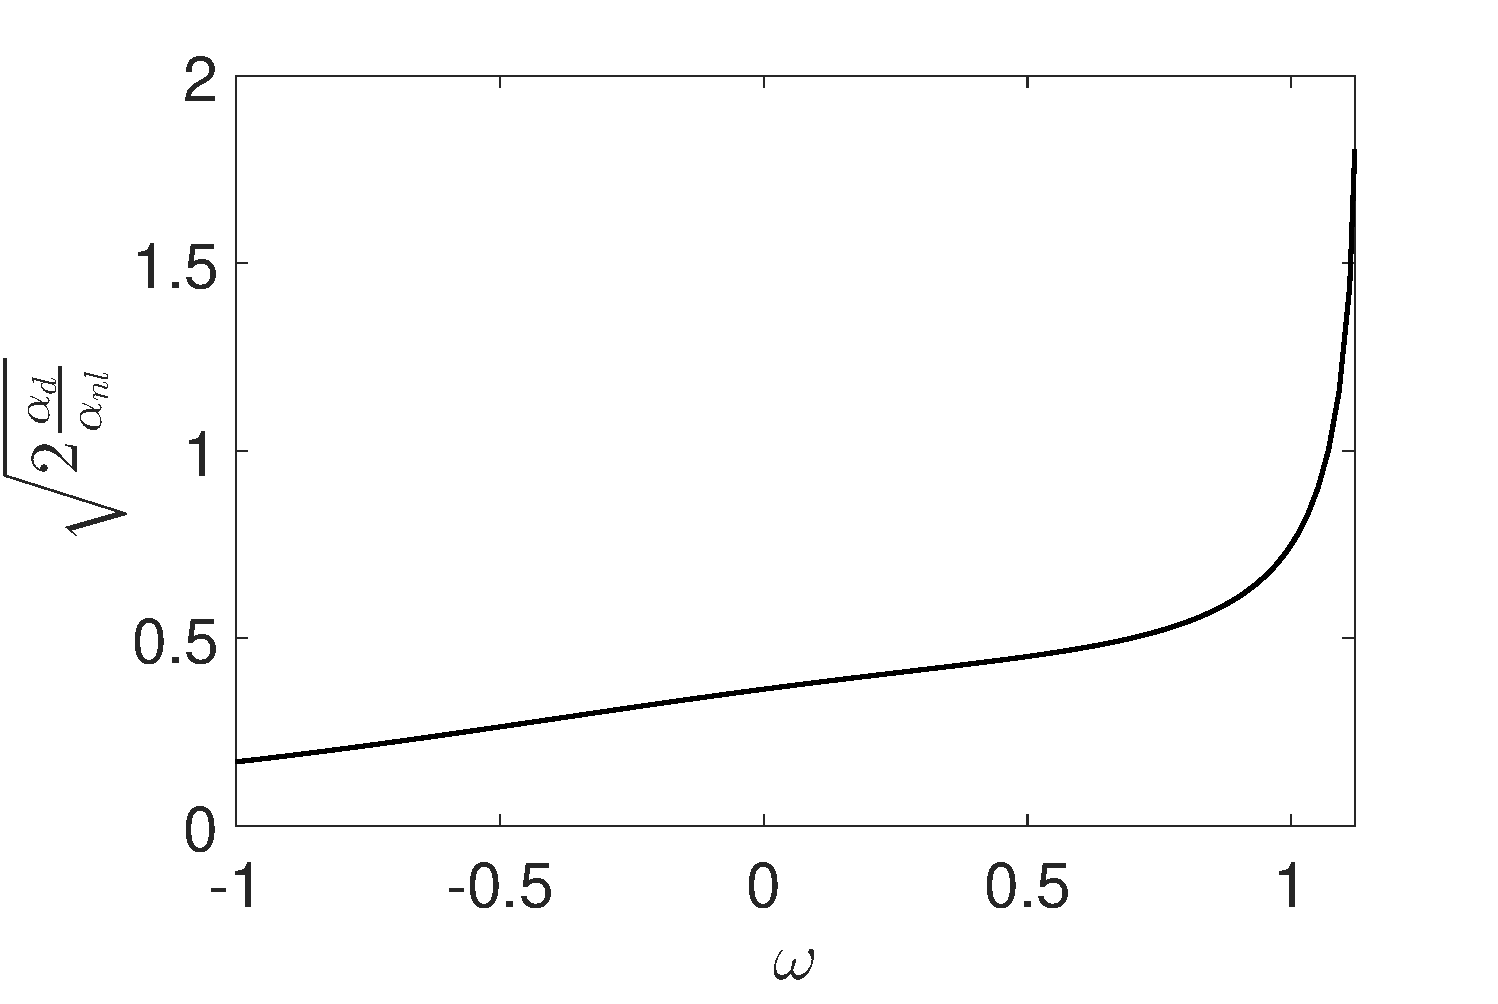
\includegraphics[width=.32\textwidth]{amp_factor_k0_1_n1_to_1pt12} & 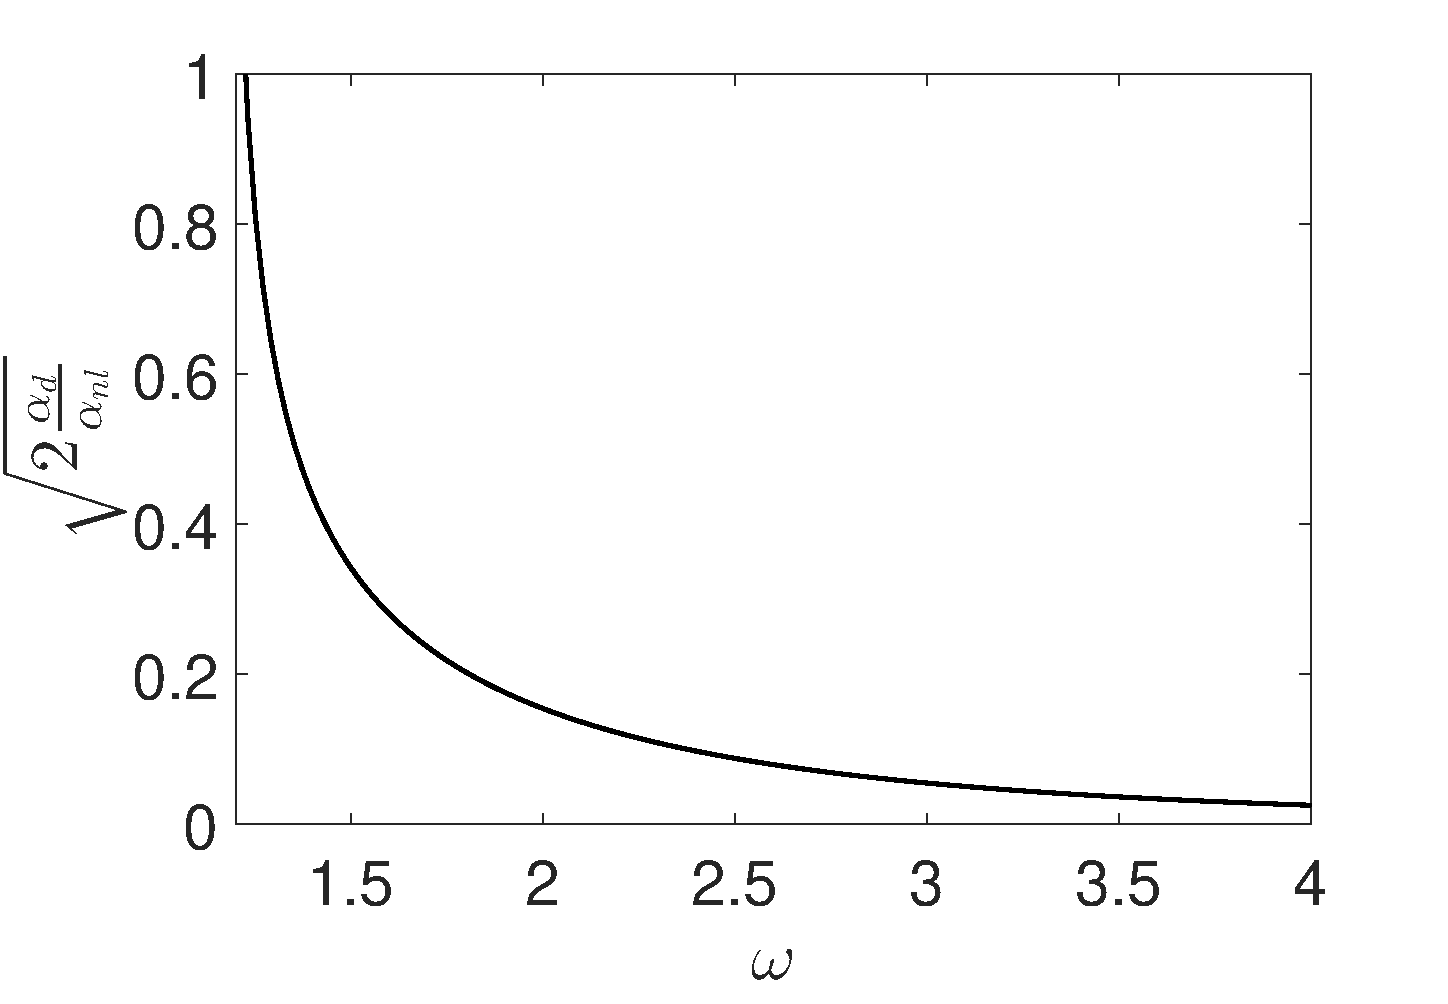
\includegraphics[width=.32\textwidth]{amp_factor_k0_1_1pt2_to_4}\\
(a) & (b) & (c)
\end{tabular}
\caption{\small Strength of the surface velocity as measured via plots of $\sqrt{2|\alpha_{d}/\alpha_{nl}|}$ for $k_{0}=1$ for $-1\leq \omega \leq 4$ (a), $-1\leq \omega \leq 1.12$ (b), and $1.17\leq \omega \leq 4$ (c).  Increasing shear increases the velocity on the focusing side, and decreases it on the defocusing side.}
\label{fig:ampcomps}
\end{figure}
In the focusing case, increasing the magnitude of the Jacobi elliptic function solutions corresponds to increasing the shear strength.  In the defocusing case, decreasing the magnitude of the Jacobi elliptic function solutions corresponds to increasing the shear strength.  These two statements are justified by the similarities of Figures \ref{fig:ampcomps} (b) and (c) and \ref{fig:stksdrfcomp} (b) and (c).  Therefore, relatively large amplitude solutions inducing strong fluid particle drift is to be expected near the resonance curve.  
%%%%%%%%%%%%%%%%%%%%%%%%%%%%%%%%%%%%%%%%%%%%%%%%%%%%%%%%%%%%%%%%%%%%%%%%%%%%%%%%%%% 
\subsection{Focusing Case}

Using the solution given in equation \eqref{cnsolns} with $k_0\approx1$ ensures that $\omega = 0$ and $\omega=\pm 1$ are in the focusing regime.   Figure \ref{fig:foc_kap_pt5} shows the paths of particles for three values of $\omega$ found by setting $\epsilon=0.1$, $\kappa=0.5$, and solving the dynamical system for the particle paths up to time $t=1/\epsilon^{2}$.  The carrier profile is propagating to the left in this situation.  Therefore, if $\omega=1.12$, then the shear current is counter-propagating at the surface with respect to the carrier wave while if $\omega=-1$, the current is co-propagating.  The counter-propagating current significantly enhances the leftward horizontal motion of a tracer along the surface as seen by comparing Figures \ref{fig:foc_kap_pt5}(b) and (c) with (a).  This can be explained by examining the values of the SDV and the LDV parameters
\[
\begin{array}{lcl}
\tilde{u}^{S}(1,0) = -0.5222, & & \tilde{u}^{L}(1,0) = -0.5222,\\
\tilde{u}^{S}(1,1.12) = -10.7373,& & \tilde{u}^{L}(1,1.12) = -5.2195,\\
\tilde{u}^{S}(1,0) = -0.2836, & & \tilde{u}^{L}(1,-1) = -0.1636,
\end{array}
\]
where the parameter $\tilde{u}^{L}$ is defined to be 
\[
\tilde{u}^{L}(k_{0},\omega) = 2\left|\frac{\alpha_{d}(k_{0},\omega)}{\alpha_{nl}(k_{0},\omega)}\right|u^{L}_{p}(k_{0},\omega).
\]
Note that for the Jacobi elliptic solutions and controlling for $\kappa$ and $\beta$, this will be the most significant contribution to the magnitude of the LDV.  This demonstrates why the counter-propagating current so enhances the leftward drift since the LDV parameter is an order of magnitude larger than in the other cases.    Further, it demonstrates why the co-propagating current, i.e. $\omega=-1$, reduces the horizontal displacement of the surface particle.  This is somewhat surprising as one might intuitively imagine that the co-propagating shear would enhance the particle drift, especially in comparison to the zero vorticity case.  However, we have effectively shown that nonlinearity makes the surface/current interaction a more complicated one than one might at first suspect.  
\begin{figure}
\centering
\begin{tabular}{cc}
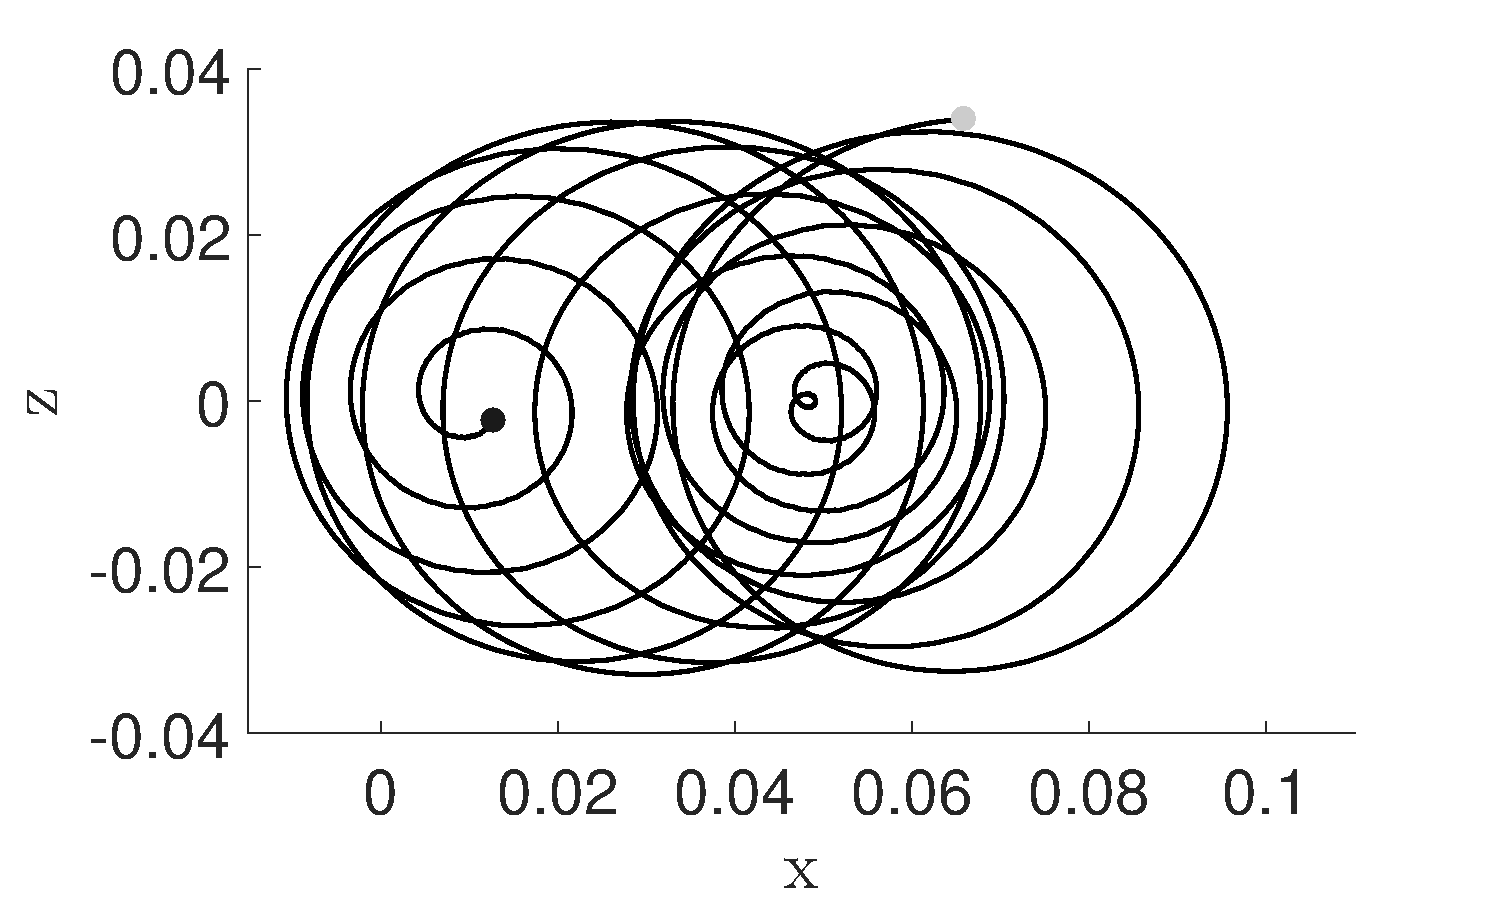
\includegraphics[width=.48\textwidth]{track_ep_pt1_tf_1_w_0_kap_pt5_foc} & 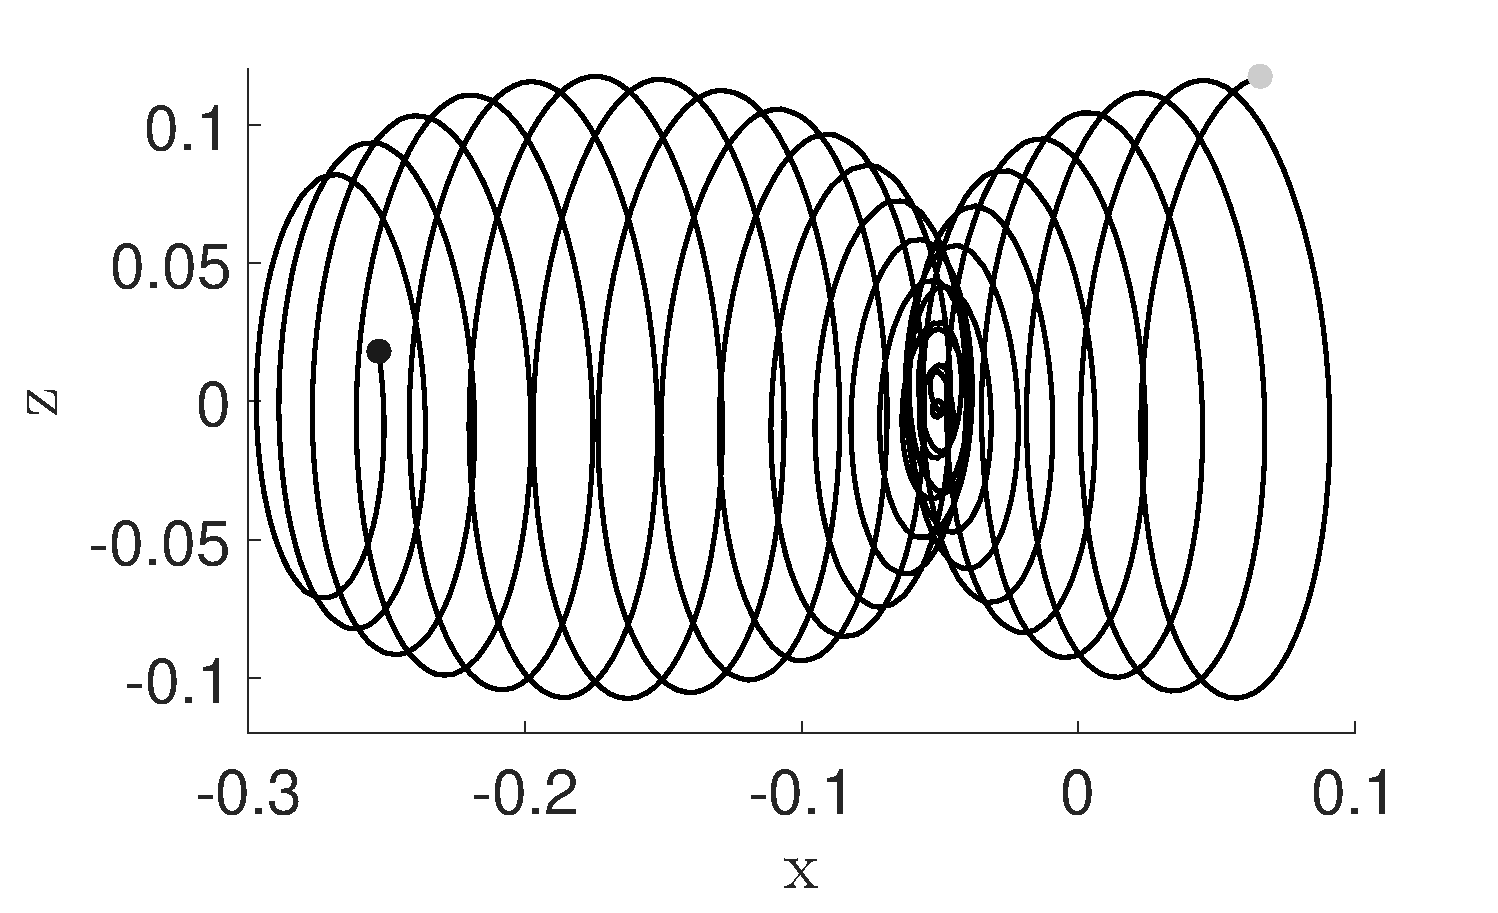
\includegraphics[width=.48\textwidth]{track_ep_pt1_tf_1_w_1pt12_kap_pt5_foc} \\
(a) & (b) \\ 
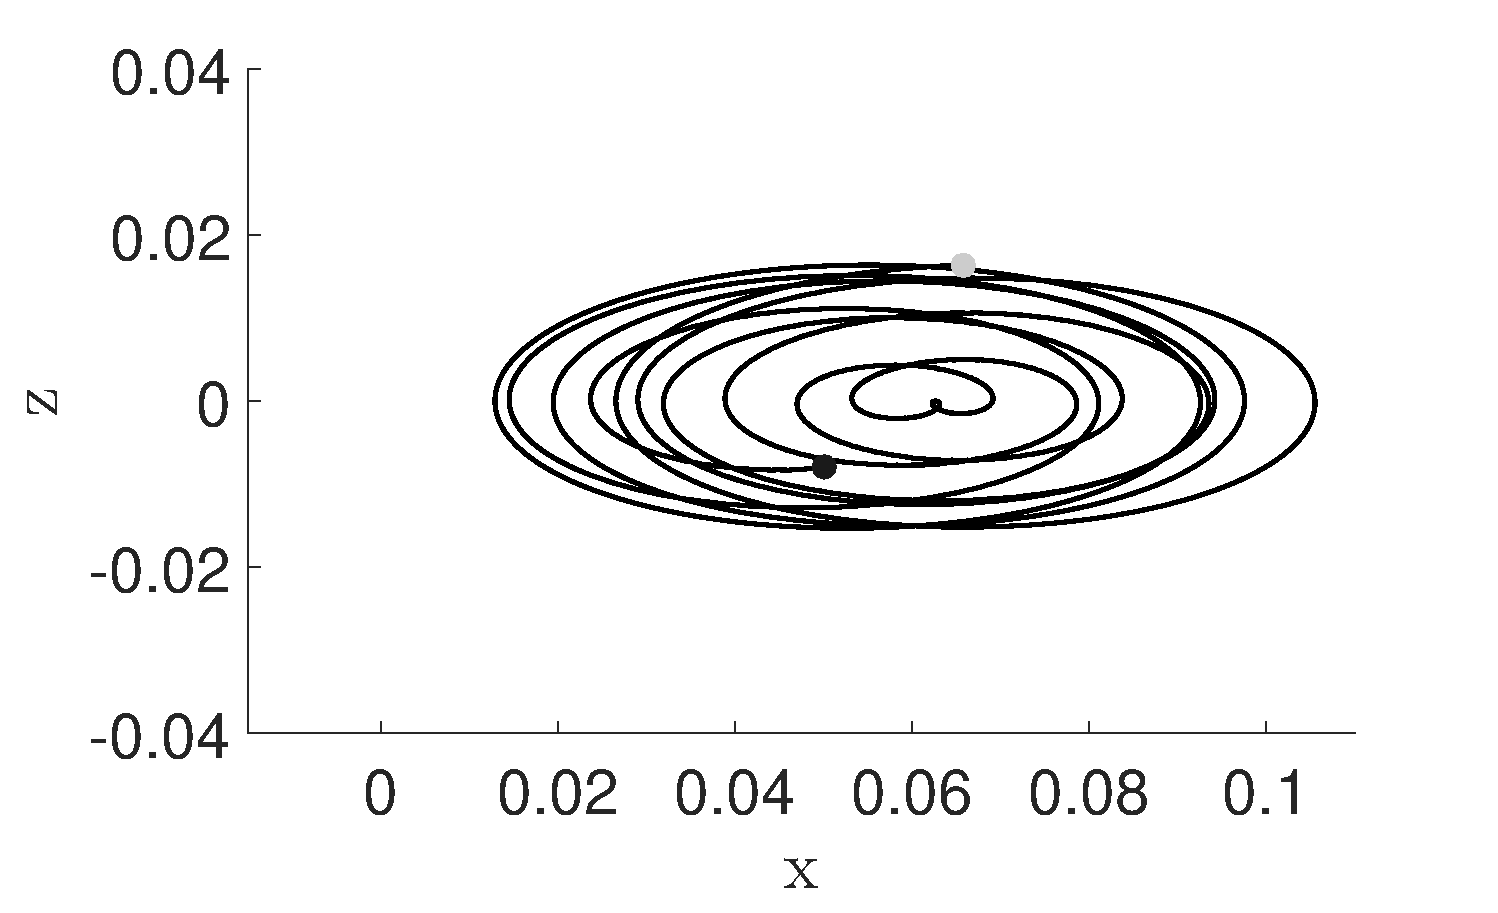
\includegraphics[width=.48\textwidth]{track_ep_pt1_tf_1_w_n1_kap_pt5_foc} & \\
(c) & 
\end{tabular}
\caption{\small {\bf Focusing Case} - Plots of particle paths correspond to the solution given in Equation (\ref{cnsolns}) with $\epsilon=0.1$, $\beta=1$, $k_{0}\approx 1$, $\kappa=0.5$, with $\omega=0$ (a), $\omega=1.12$ (b), and $\omega=-1$ (c). The grey dots indicate the starting positions of the tracers while the black dots indicate their final positions.}
\label{fig:foc_kap_pt5}
\end{figure}

Choosing $\kappa=0.99$ shows that similar results hold closer to the solitary wave solution; see Figure \ref{fig:foc_kap_pt99}, though the larger elliptic modulus results in the larger amplitudes and leftward drifts.  In particular, near the solitary wave limit, positive, counter-propagating shear can greatly enhance both the impact of nonlinearity and the transport properties of the waves.    
\begin{figure}
\centering
\begin{tabular}{cc}
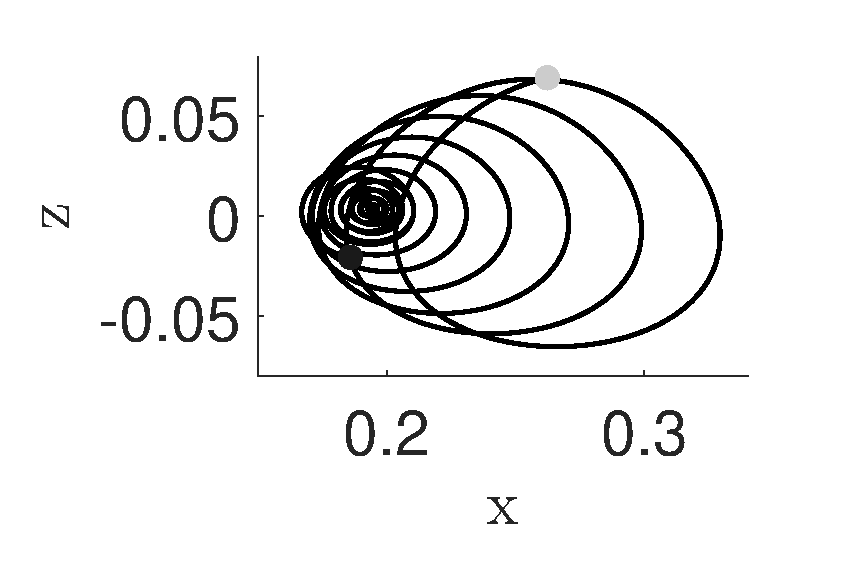
\includegraphics[width=.48\textwidth]{track_ep_pt1_tf_1_w_0_kap_pt99_foc} & 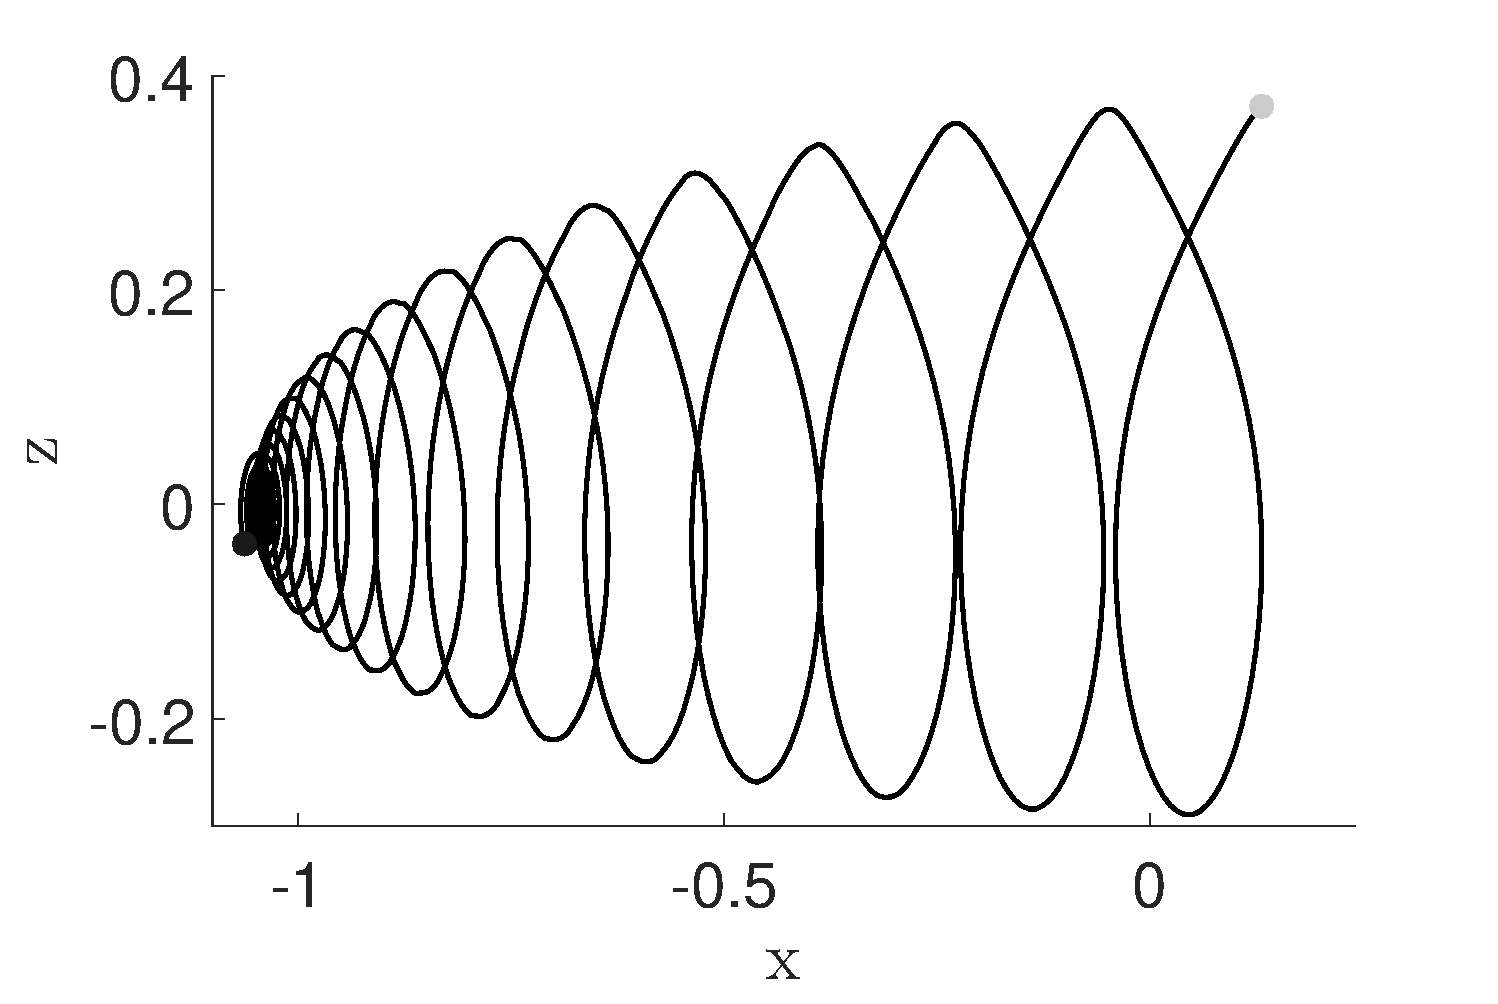
\includegraphics[width=.48\textwidth]{track_ep_pt1_tf_1_w_1pt12_kap_pt99_foc} \\
(a) & (b) \\ 
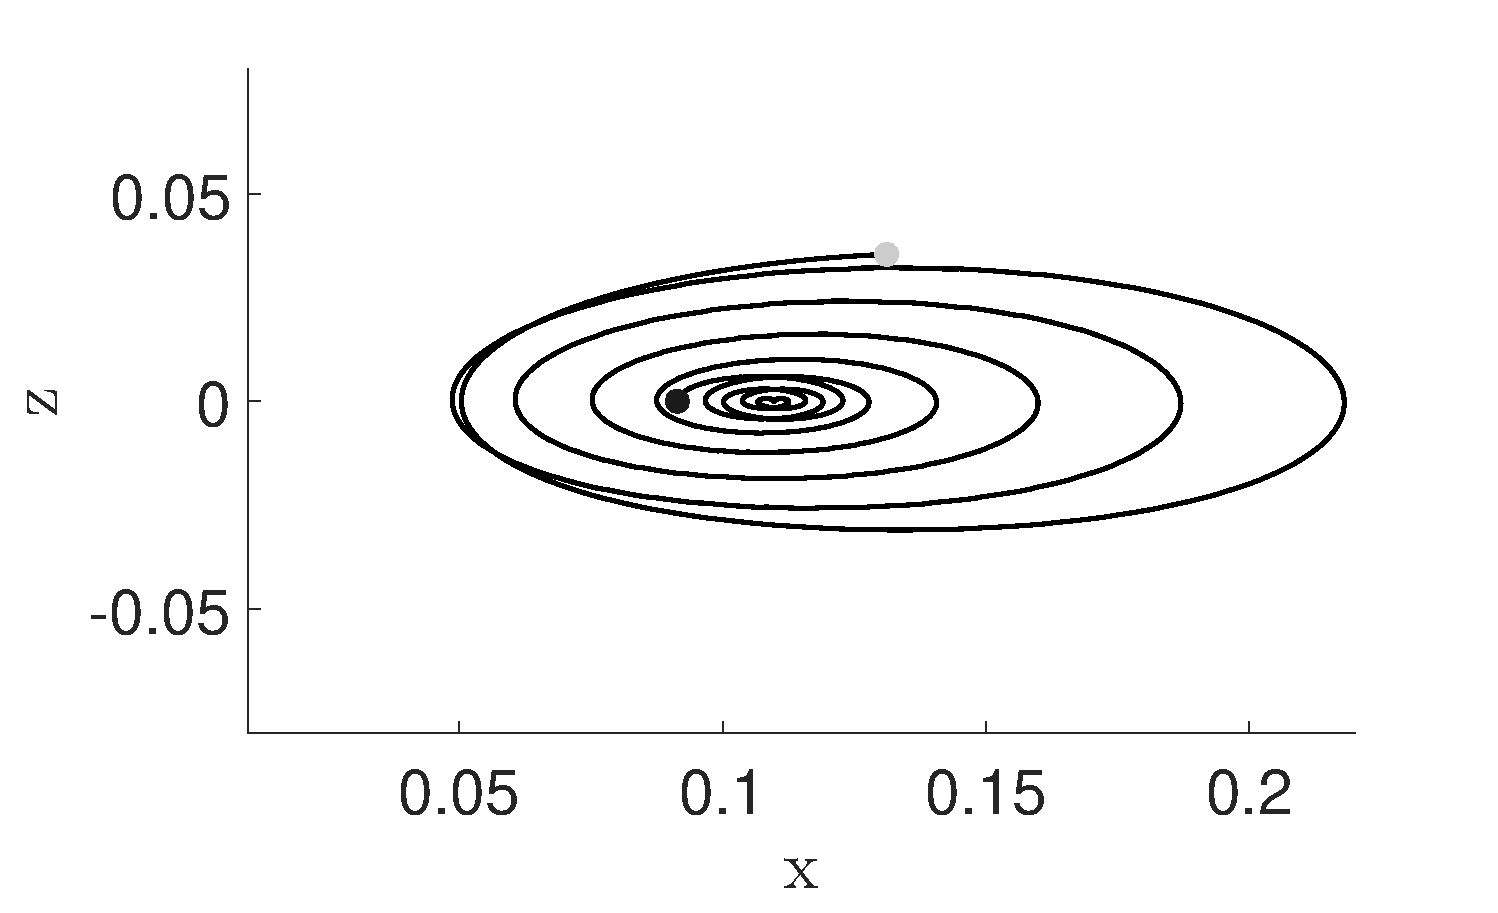
\includegraphics[width=.48\textwidth]{track_ep_pt1_tf_1_w_n1_kap_pt99_foc} & \\
(c) & 
\end{tabular}
\caption{\small {\bf Focusing Case} - Plots of particle paths correspond to the solution given in Equation (\ref{cnsolns}) with $\epsilon=0.1$, $\beta=1$, $k_{0}\approx 1$, $\kappa=0.99$, with $\omega=0$ (a), $\omega=1.12$ (b), and $\omega=-1$ (c). The grey dot indicates the starting position of the tracer while the black dot indicates the final position.}
\label{fig:foc_kap_pt99}
\end{figure}

%%%%%%%%%%%%%%%%%%%%%%%%%%%%%%%%%%%%%%%%%%%%%%%%%%%%%%%%%%%%%%%%%%%%%%%%%%%%%%%%%%%
\subsection{Defocusing Case}

For the Jacobi elliptic solutions with $k_{0}\approx 1$, the zero LDV solutions belong in the defocusing case.  Figure \ref{fig:jaczerodrift} shows the impact on surface flow particle paths when $\omega$ is chosen to zero out the LDV.
\begin{figure}
\centering
\begin{tabular}{cc}
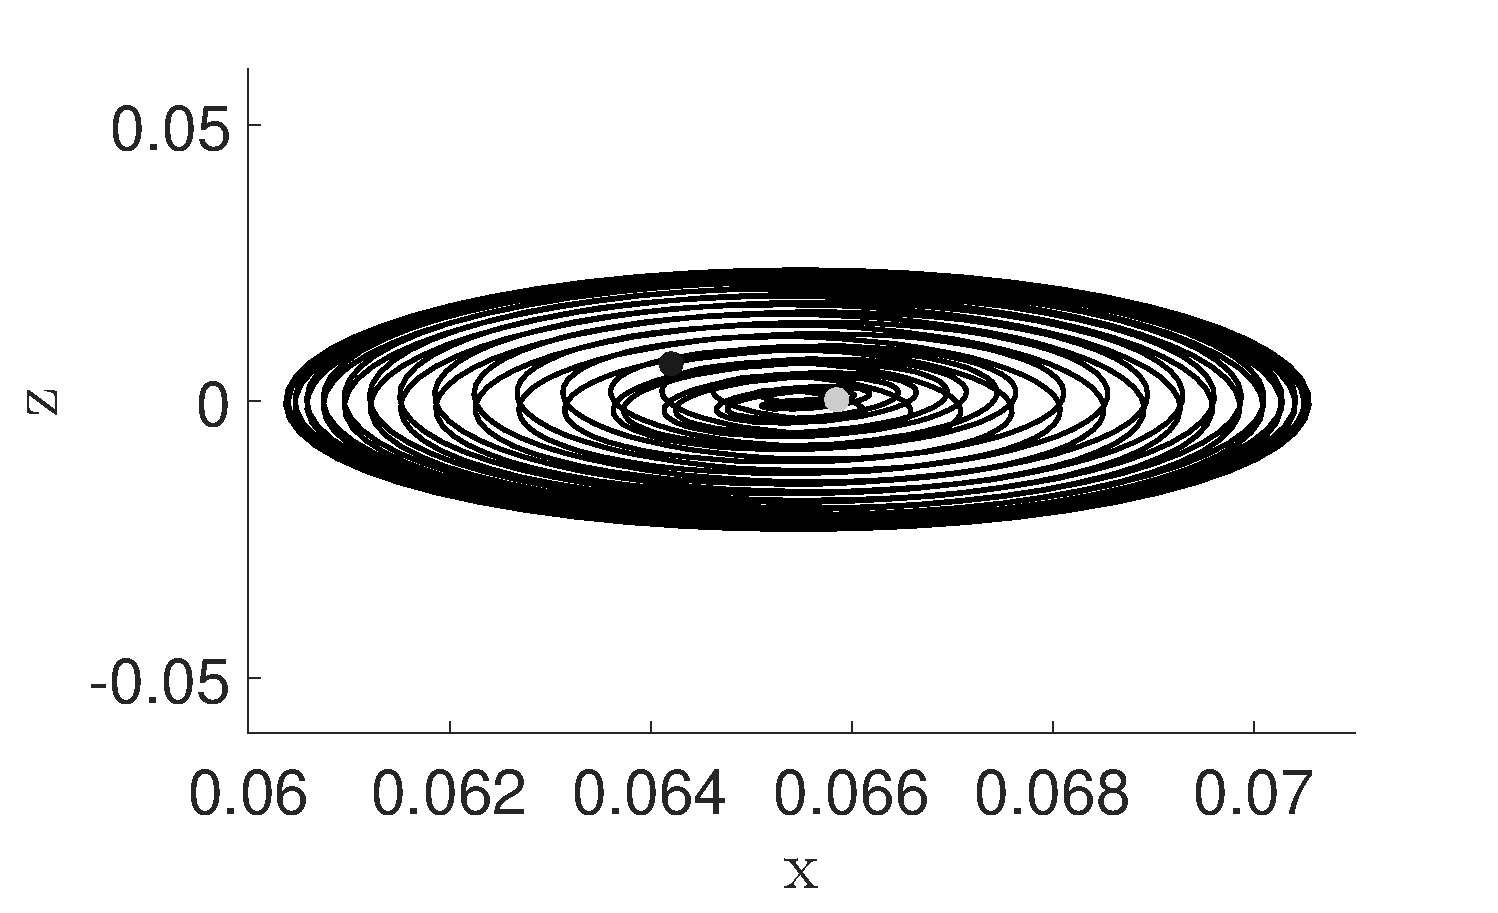
\includegraphics[width=.48\textwidth]{track_ep_pt1_tf_1_w_1pt704_kap_pt5_foc} & 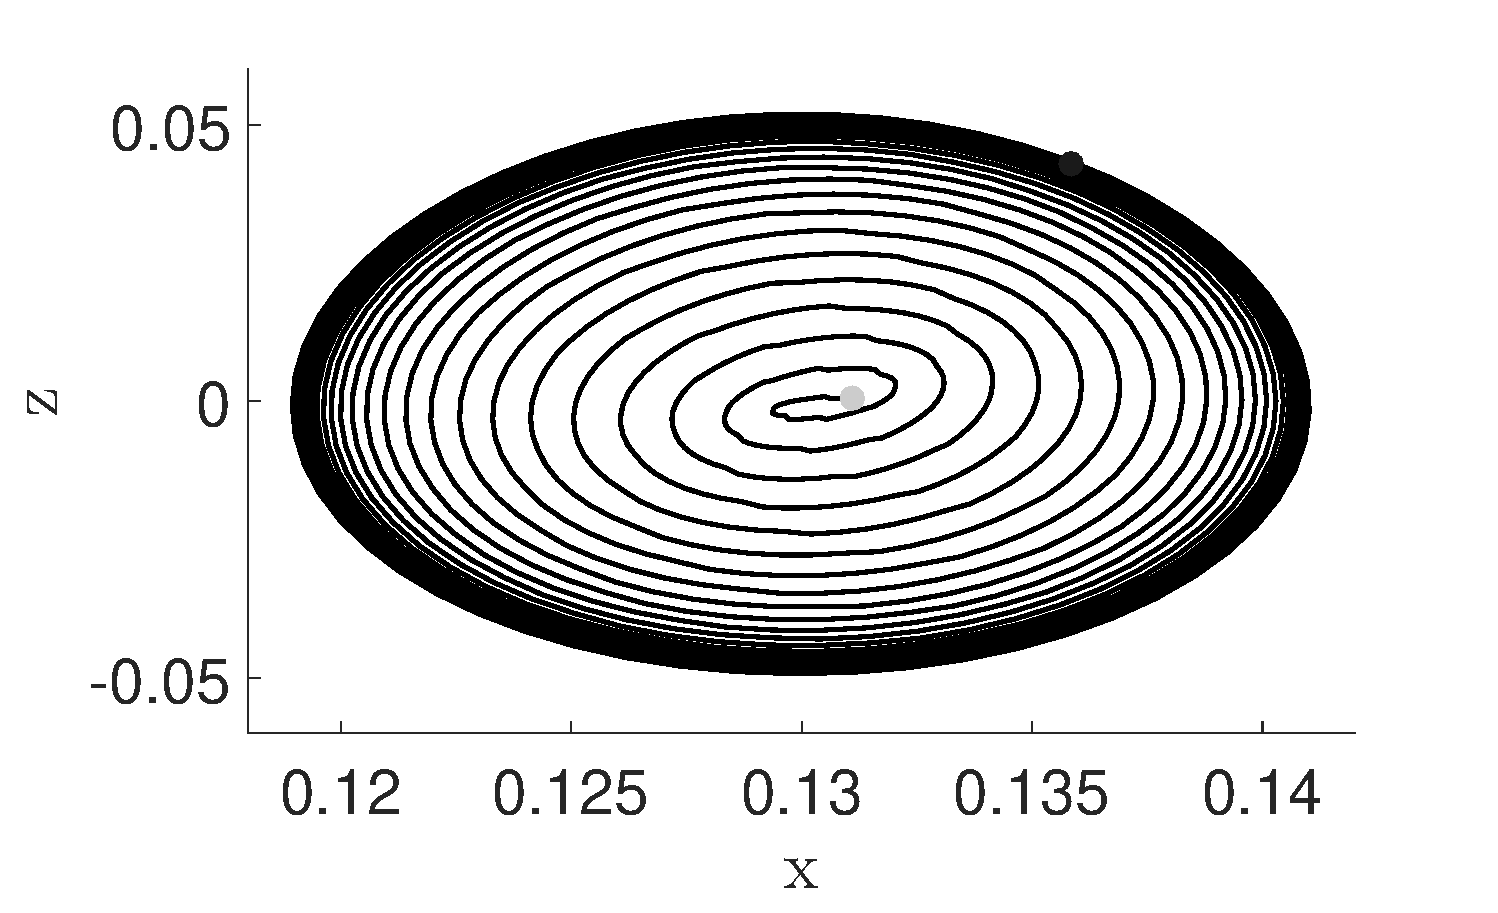
\includegraphics[width=.48\textwidth]{track_ep_pt1_tf_1_w_1pt668_kap_pt99_foc} \\
(a) $\omega=1.7037$ & (b) $\omega=1.6682$ 
\end{tabular}
\caption{\small {\bf Defocusing Case} - Plots of particle paths correspond to the solution given in Equation (\ref{snsolns}) with $\epsilon=0.1$, $\beta=1$, $k_{0}\approx 1$, with $\kappa=0.5$  (a), $\kappa=0.99$ (b). The grey dots indicate the starting positions of the tracers while the black dots indicate their final positions.  }
\label{fig:jaczerodrift}
\end{figure}
As can be seen, the particle paths, while not exactly closed, are spirals and are constrained in their horizontal and vertical extent by an outer elliptical perimeter.  Similarly, the shear strength can be chosen so that the LDV is zeroed out for the plane-wave solutions.  Taking $k_{0}=1$ and $A=1$, this corresponds to choosing $\omega = 1.6828$.  Figure \ref{fig:pwavezdrift} shows a nearly closed particle path.  We emphasize that these results are a confirmation of the predictions made in Figure \ref{fig:zerodriftk0}.  Thus, these numerical results validate our choice to generalize the GLM approach in so far as we see the generalization provides the correct predictions for when shear will quench surface drift.
\begin{figure}
\centering
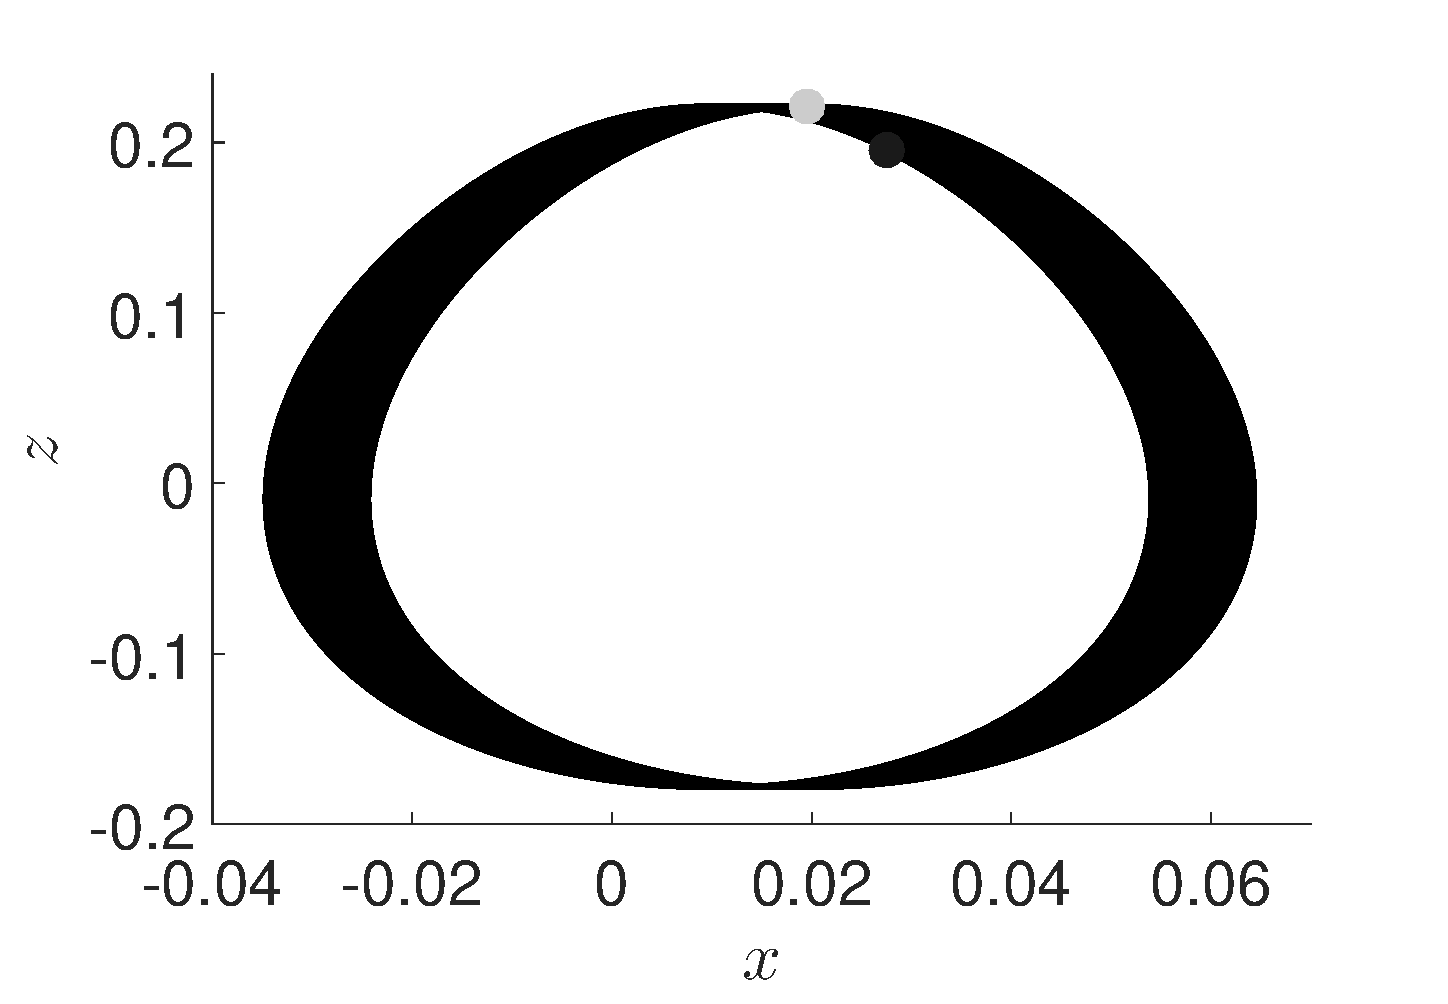
\includegraphics[width=.48\textwidth]{om_val_1pt7_k0_1_ep_pt1_defoc_ztrack_pwave}
\caption{\small {\bf Defocusing Case} - Plot of a particle path corresponding to a plane-wave solution with $\epsilon=0.1$, $A=1$, $k_{0}=1$ , and $\omega=1.6828$, which ensures that $\tilde{u}^{L}(1,\omega)=0$, thereby leading to the nearly closed particle path.}
\label{fig:pwavezdrift}
\end{figure}  

In some respects then, we have also shown that by appropriately choosing the shear, we can replicate the dynamics of a Gerstner wave \cite{constantin} by looking instead at a plane-wave moving over a counter-propagating shear current.  This could point towards resolving some of the questions raised in \cite{monismith,smith}, though this is a subject of future research.  

Looking beyond cases in which Eulerian counterflows quench drift, we now consider the defocusing NLS Jacobi elliptic function solutions given in Equation \eqref{snsolns}.  We choose $k_{0}\approx1$, $\epsilon=0.1$, $\kappa=0.99$ (near the dark-soliton limit).  Solving the dynamical system for the particle paths up to time $t=1/\epsilon^{2}$ generates Figure \ref{fig:defoc_kap_pt99} (a) and (b) for $\omega= 1.17$ and $\omega= 4$ respectively.  While the particle path motion seen in Figure \ref{fig:defoc_kap_pt99}(a) is rapidly oscillating, the net transport and amplitude is quite small.
\begin{figure}
\centering
\begin{tabular}{cc}
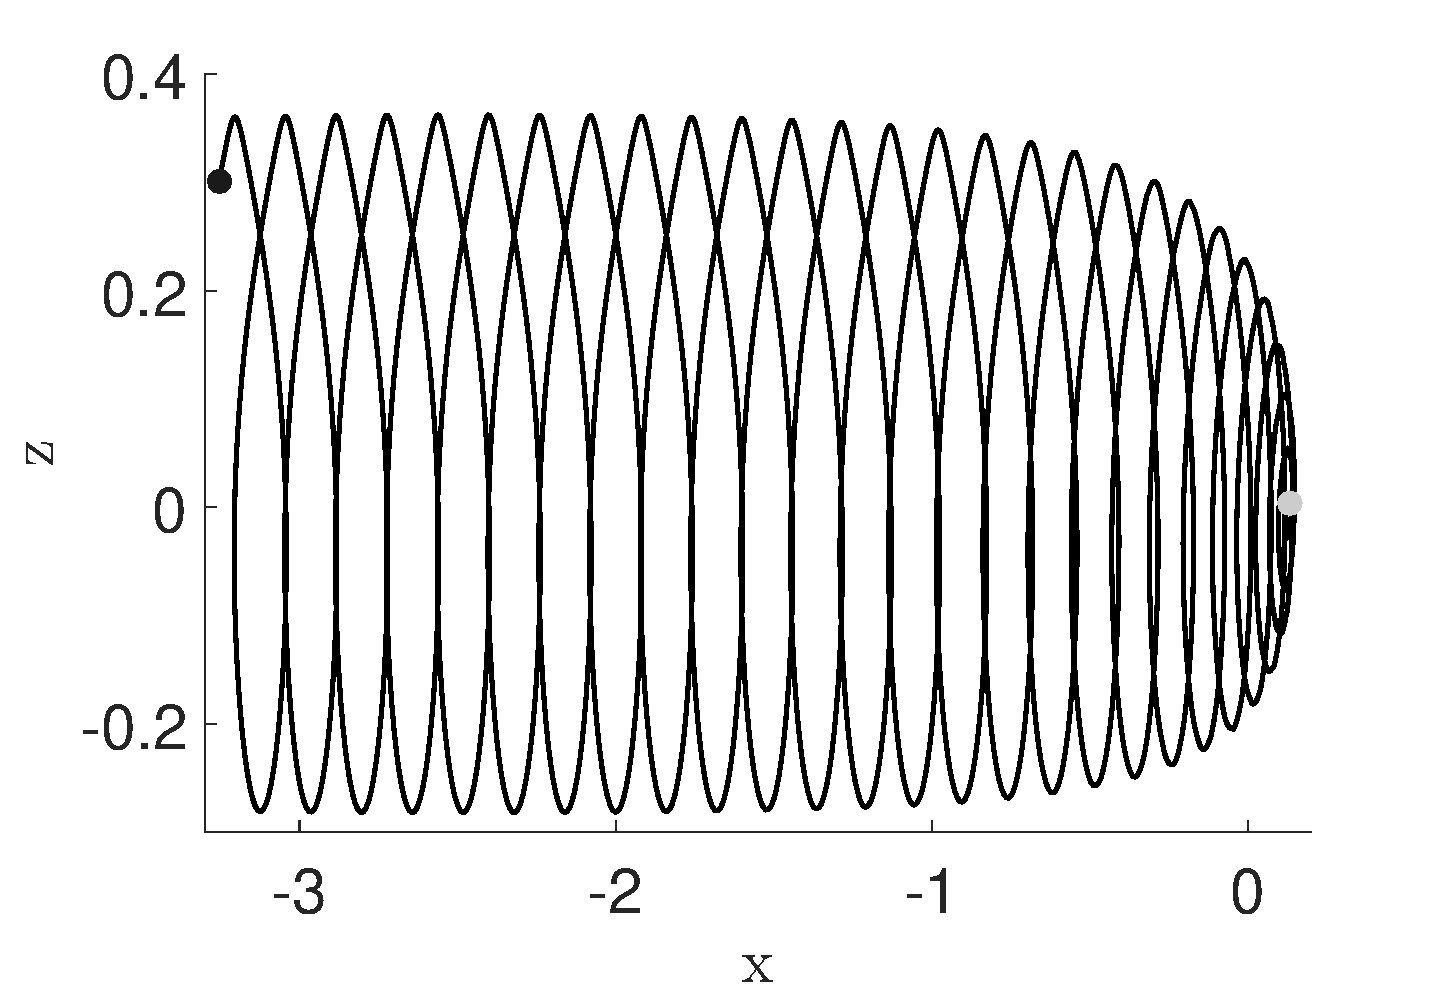
\includegraphics[width=.48\textwidth]{om_val_1pt17_k0_1_ep_pt1_defoc_ztrack} &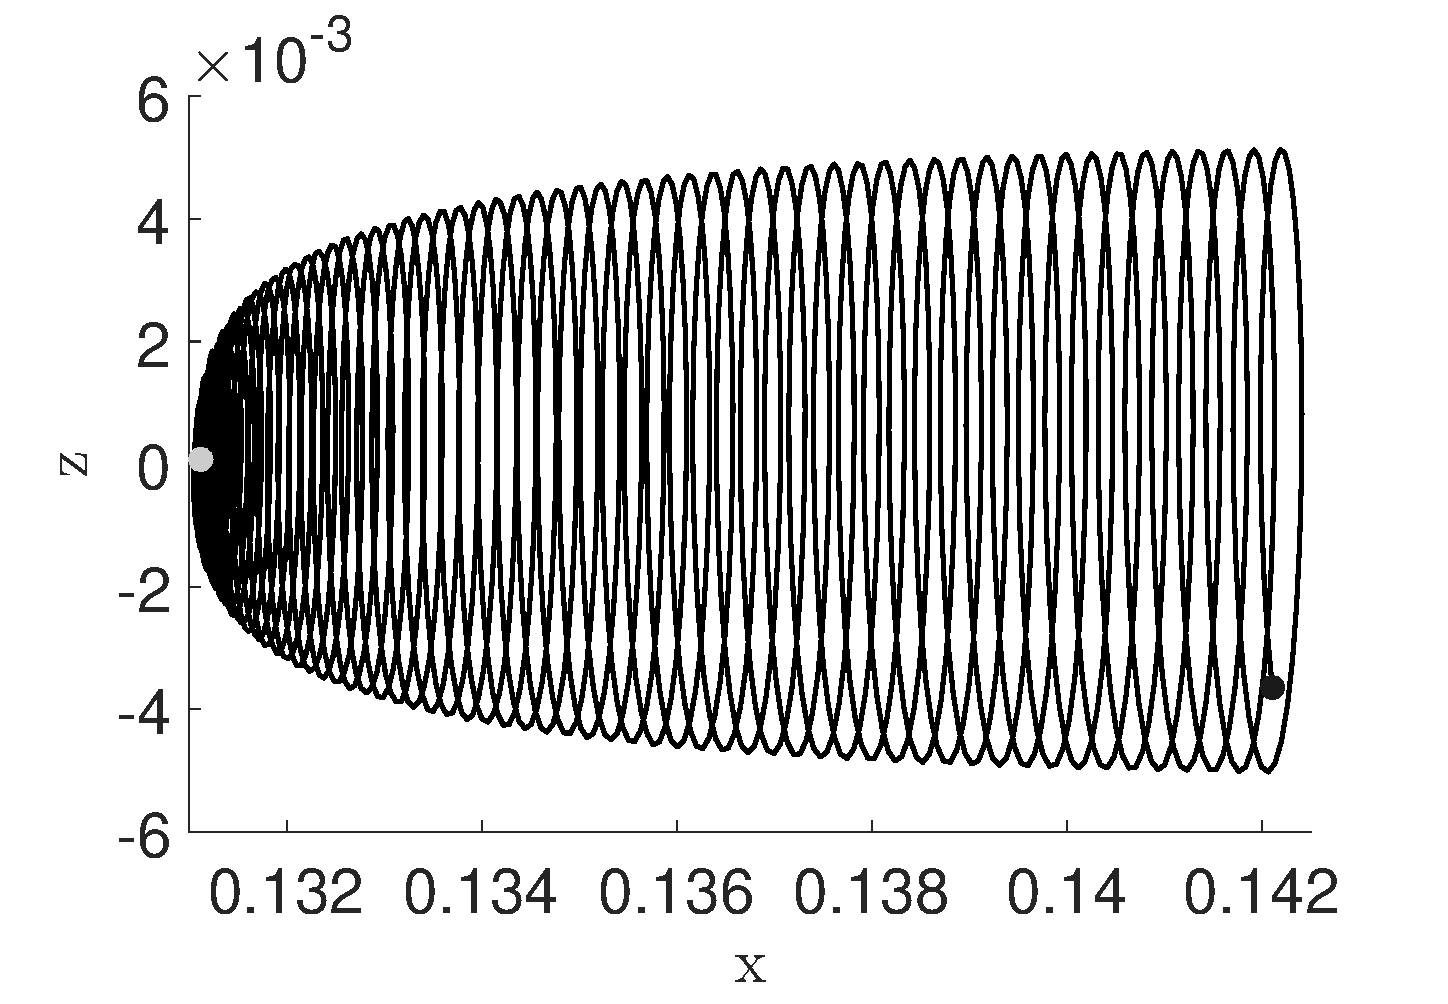
\includegraphics[width=.48\textwidth]{om_val_4_k0_1_ep_pt1_defoc_ztrack} \\
(a) $\omega = 1.17$ & (b) $\omega=4$
\end{tabular}
\caption{\small {\bf Defocusing} - Near dark soliton solution for $k_{0}\approx1$, $\kappa=.99$ and $\omega=1.17$ (a) and $\omega=4$ (b).  The grey dot indicates the starting position of the tracer while the black dot indicates the final position.}
\label{fig:defoc_kap_pt99}
\end{figure}

However, if $\omega=4$ in the case of a plane wave, we do not necessarily get the same diminished response seen for the Jacobi elliptic solutions; see Figure \ref{fig:defoc_pwave}.  The highly oscillatory plane wave profile induces a particle path which ultimately exhibits a strong rightward drift which follows the strong counter-propagating shear current.   Using Equations \eqref{lagrandrift} and \eqref{pwavesdrift}, and expanding around $z=\epsilon \eta$, the associated SDV and LDV at the surface for the plane wave with these parameters are given by 
\begin{align*}
u^{S} = & -8.9452\epsilon^{2} + \mathcal{O}(\epsilon^{3}),\\
\bar{u}^{L} = & 28.7778\epsilon^{2} + \mathcal{O}(\epsilon^{3}).
\end{align*}
This explains the stronger net rightward drift of the particle shown in Figure \ref{fig:defoc_pwave}.  Finally, note that this shows the SDV and the LDV can oppose one another, thereby clarifying the need to use both velocities to fully understand the drift properties associated with a surface wave.  
 \begin{figure}
\centering
\begin{tabular}{cc}
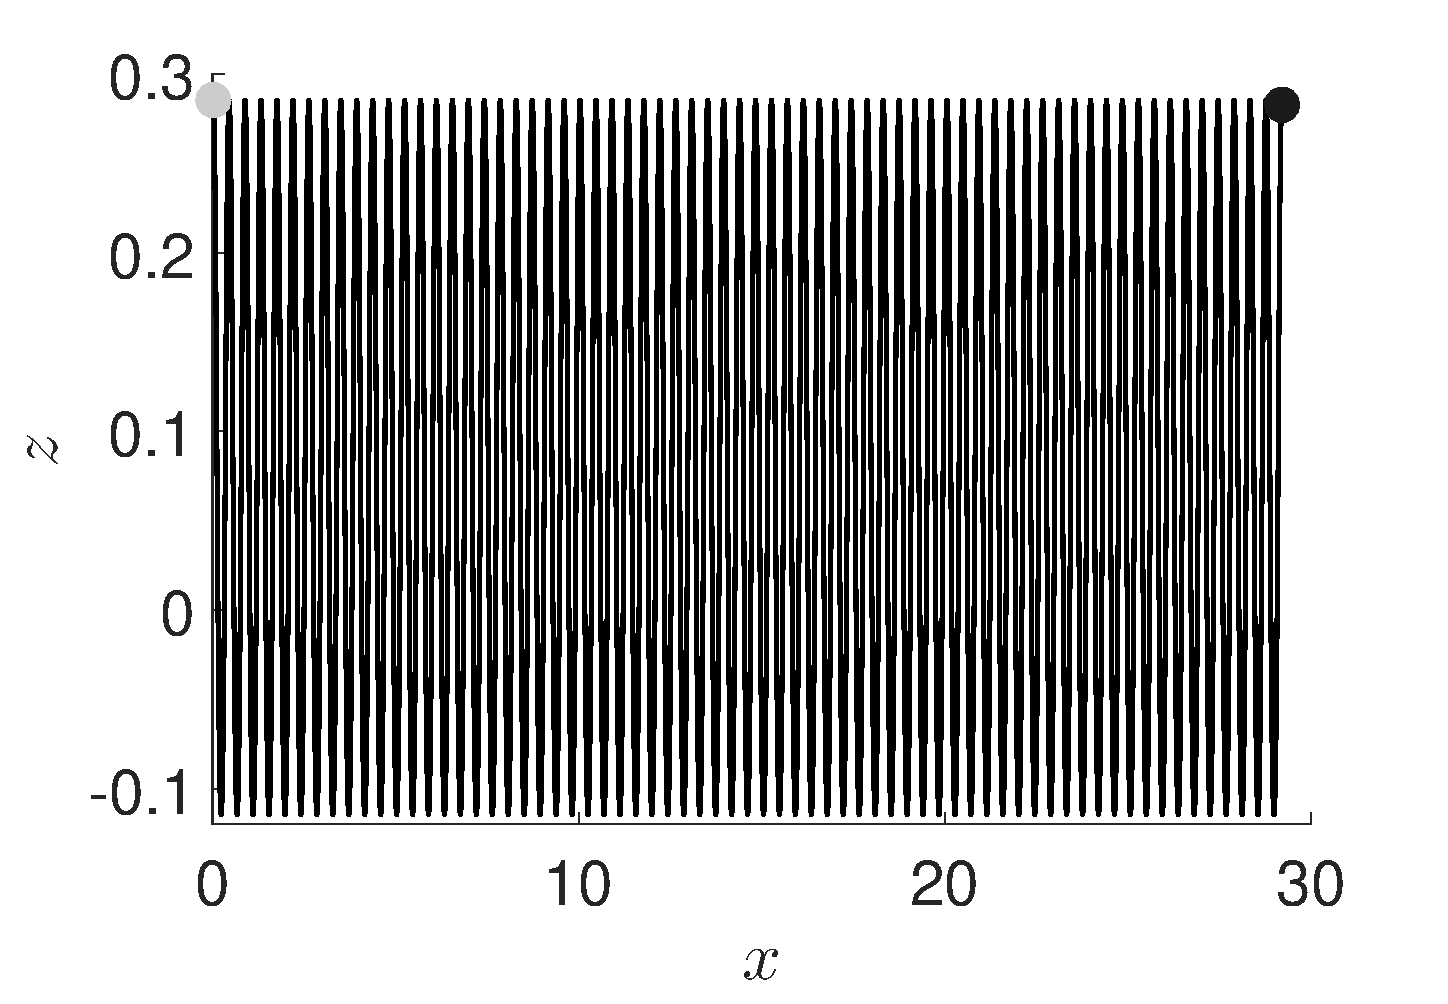
\includegraphics[width=.5\textwidth]{om_val_4_k0_1_ep_pt1_defoc_ztrack_pwave} & 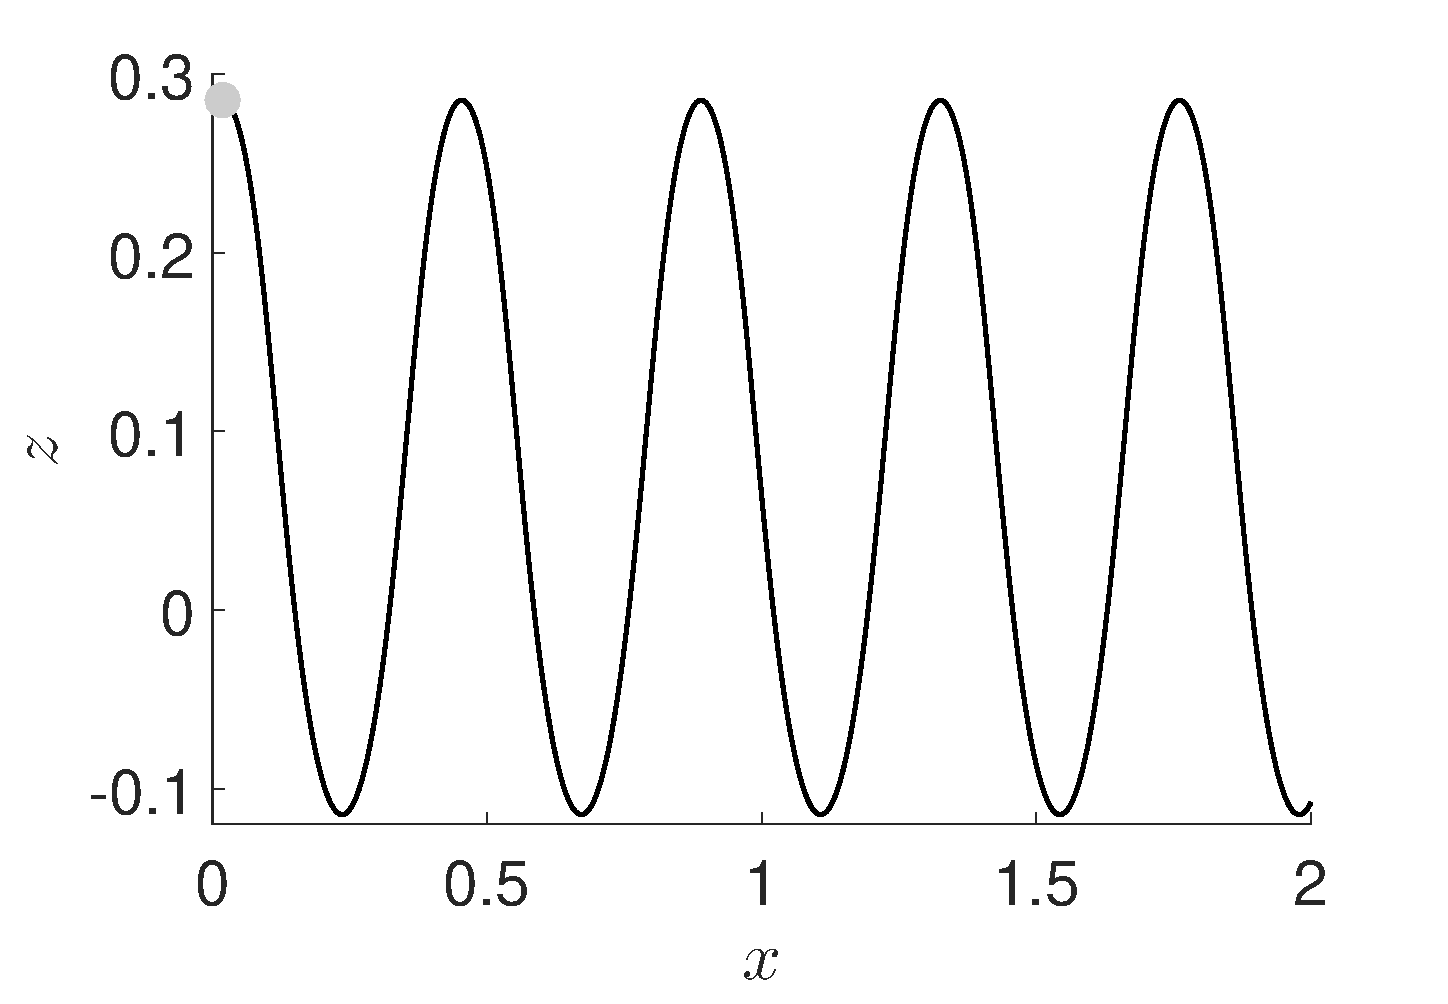
\includegraphics[width=.5\textwidth]{om_val_4_k0_1_ep_pt1_defoc_ztrack_pwave_detail}\\
(a) & (b)
\end{tabular}
\caption{\small {\bf Defocusing Case} - Plane-wave solution for $k_{0}=1$, $\omega=4$, $A=1$, with (b) providing a detail of (a).  The grey dot indicates the starting position of the tracer while the black dot indicates the final position.}
\label{fig:defoc_pwave}
\end{figure}

\section{Conclusion and Future Directions}

\section{Acknowledgments}
This material is based upon work supported by the National Science Foundation under Grant No. DMS-1439786 while CWC and JDC were in residence at the Institute for Computational and Experimental Research in Mathematics in Providence, RI, during the Spring 2017 semester.  Additionally, JDC acknowledges and thanks the Norwegian Fulbright Core Scholar Program for supporting his five-month long visit to the University of Bergen to work with HK. This research was also supported by
the Research Council of Norway through grants 213474/F20 and 239033/F20.

\bibliographystyle{JFM_Style/jfm}
\bibliography{deep_water_shear}
\end{document}